\documentclass[11pt]{article}
\usepackage{amsmath, amssymb, amscd, amsthm, amsfonts}
\usepackage{graphicx}
\usepackage{hyperref}
\usepackage{algorithm}  
\usepackage{algpseudocode} 
\usepackage{makecell}
\usepackage{amsmath}
\usepackage{enumitem}
\usepackage{graphicx}    % For including images
\usepackage{subfigure}
\usepackage{subcaption}  % For subfigures
\usepackage{caption}     % For customizing captions (optional)
\usepackage{float}       % For controlling figure placement (optional)

\setcellgapes[t]{0pt}
\setlength\extrarowheight{0pt}
\makegapedcells 
\oddsidemargin 0pt
\evensidemargin 0pt
\marginparwidth 40pt
\marginparsep 10pt
\topmargin -20pt
\headsep 10pt
\textheight 8.7in
\textwidth 6.65in
\linespread{1.2}
\usepackage{enumerate}
\usepackage{amsfonts,amsmath,amsthm,amssymb}
\newtheorem{corollary}{Corollary}



\usepackage[textsize=tiny]{todonotes} % To-do notes

\newcommand{\todoyp}[2][]{\todo[size=\scriptsize,color=green!20!white,#1]{Yiping Lu: #2}}
\usepackage[most]{tcolorbox}
\tcbuselibrary{theorems}

\usepackage[most]{tcolorbox}
\usepackage{framed}
\usepackage{xcolor}
\usepackage{bm}
\colorlet{shadecolor}{orange!15}

\tcbset{
    mymathstyle/.style={
        colback=cyan!10,    % 背景颜色
        colframe=cyan!50,   % 边框颜色
        sharp corners,      % 去掉圆角
        boxrule=0.5pt,      % 边框粗细
        left=2pt,           % 左侧内边距
        right=2pt,          % 右侧内边距
        top=2pt,            % 上边内边距
        bottom=2pt          % 下边内边距
    }
}

\usepackage{mdframed}  % For creating framed environments

% Define a custom environment "warningbox" with a colored/shadowed frame
\newmdenv[
  backgroundcolor=yellow!20,
  linecolor=red,
  linewidth=2pt,
  roundcorner=10pt,
  shadow=true,
  nobreak=true
]{warningbox}

\usepackage{empheq}
\newcommand{\highlight}[1]{%
    \colorbox{cyan!10}{$\displaystyle #1$}%
}

\include{thm}

\title{What is a Sketch-and-Precondition Derivation for Low-Rank Approximation? Inverse Power Error or Inverse Power Estimation?}
\author{Ruihan Xu \thanks{Department of Mathematics, University of Chicago, email:\texttt{ruihanx@uchicago.edu}} \and Yiping Lu \thanks{Industrial Engineering \& Management Science, Northwestern University, email: \texttt{yiping.lu@northwestern.edu} }}
\date{}

\newtheorem{theorem}{Theorem}
\newtheorem{lemma}[theorem]{Lemma}
\newtheorem{conjecture}[theorem]{Conjecture}

\newcommand{\rr}{\mathbb{R}}

\newcommand{\al}{\alpha}
\DeclareMathOperator{\conv}{conv}
\DeclareMathOperator{\aff}{aff}
\newcommand{\yplu}[1]{{\color{orange}{ [\textbf{Yiping:}} #1]}}
\newcommand{\rh}[1]{{\color{red}{ [\textbf{Ruihan:}} #1]}}
\begin{document}

\maketitle

\begin{abstract}
Randomized sketching accelerates large-scale numerical linear algebra by reducing computational complexity. While the traditional sketch-and-solve approach reduces the problem size directly through sketching, the sketch-and-precondition method leverages sketching to construct a computational friendly preconditioner. This preconditioner improves the convergence speed of iterative solvers applied to the original problem, maintaining accuracy in the full space. Furthermore, the convergence rate of the solver improves at least linearly with the sketch size. Despite its potential, developing a sketch-and-precondition framework for randomized algorithms in low-rank matrix approximation remains an open challenge. We introduce the \emph{Error-Powered Sketched Inverse Iteration} (\textbf{\texttt{EPSI}}) Method via run sketched Newton iteration for the Lagrange form as a sketch-and-precondition variant for randomized low-rank approximation. Our method achieves theoretical guarantees, including a convergence rate that improves at least linearly with the sketch size.
\end{abstract}

\begin{center}
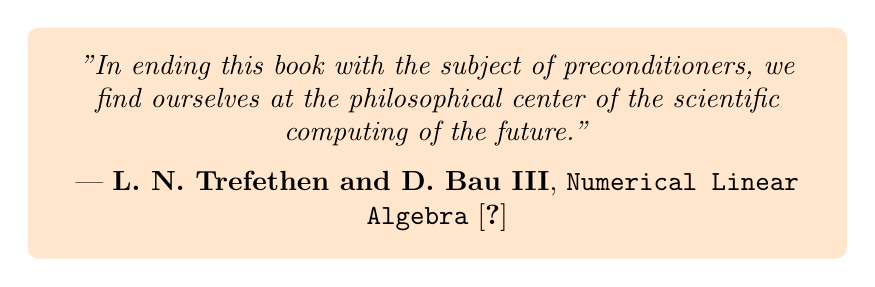
\begin{tikzpicture}
    % node options:
    %   fill=orange: background color
    %   fill opacity=0.5: semi-transparency
    %   text opacity=1: text remains fully opaque
    %   rounded corners: round the corners of the box
    %   inner sep=10pt: padding inside the box
    \node[
        fill=orange,
        fill opacity=0.2,
        text opacity=1,
        rounded corners,
        inner sep=10pt
    ]{
        \parbox{0.8\linewidth}{
            \centering
            \emph{"In ending this book with the subject of preconditioners, 
            we find ourselves at the philosophical center of the scientific 
            computing of the future."} 
            
            \vspace{6pt}
            
            --- \textbf{L. N. Trefethen and D. Bau III}, \texttt{Numerical Linear Algebra} \cite{trefethen2022numerical}
        }
    };
\end{tikzpicture}
\end{center}

\tableofcontents

\begin{warningbox}
\textbf{Warning (First Version):} \\
We are the first version of this preprint, 
and we use the most naïve approach to prove the theorem. 
We believe the proof can be further simplified, 
and we are actively working on it.
\end{warningbox}

\section{Introduction}\label{section-introduction}

Randomized Numerical Linear Algebra (RNLA) \cite{halko2011finding,martinsson2020randomized,woodruff2014sketching,mahoney2011randomized,drineas2016randnla,murray2023randomized,avron2010blendenpik} is a rapidly advancing area of matrix computations that has significantly impacted low-rank approximations, iterative methods, projections and etc. This field highlights the power of randomized algorithms as highly effective tools for constructing approximate matrix computations. These algorithms stand out for their simplicity, efficiency, and their ability to yield surprisingly accurate results. Effective randomized least-squares solvers for minimizing $\|Ax-b\|$ ($A \in \mathbb{R}^{m \times n}$, $x \in \mathbb{R}^n$, $b \in \mathbb{R}^m$) often involve constructing a preconditioner using a sketched matrix. Notable methods include \texttt{sketch-and-precondition} approaches \cite{rokhlin2008fast, avron2010blendenpik,spielman2014nearly,meng2014lsrn,lacotte2020effective}, \texttt{iterative sketching} techniques \cite{pilanci2016iterative, ozaslan2019iterative} (with their preconditioning effect formally analyzed in \cite{xu2024randomized}), and \texttt{sketch-and-projection} frameworks \cite{gower2016sketch,gower2021adaptive} (with their preconditioning effect formally analyzed in \cite{derezinski2024sharp}). These approaches often achieve convergence rates that scale at least linearly with the sketch size, and can exhibit even faster convergence when the data matrix has favorable spectral decay properties \cite{derezinski2024sharp}.

In this paper, we mainly focus on developing a \texttt{Sketch-and-Precondition} derivation of randomized low-rank matrix approximation algorithms, which play a central role in data analysis and scientific computing. One of the most significant techniques in this area is \texttt{Randomized SVD} \cite{liberty2007randomized, halko2011algorithm, witten2015randomized, martinsson2011randomized, swartworth2023optimal}, which reduces the problem size by projecting the original matrix onto a lower-dimensional subspace using random sketching methods. The accuracy of the resulting low-rank approximation can be significantly improved through several refinement steps employing subspace iteration techniques \cite{rokhlin2010randomized, musco2015randomized, gu2015subspace,feng2024algorithm}. Such an algorithm operates as a \texttt{sketch-and-solve} approach \cite{sarlos2006improved,clarkson2017low}, where the matrix is first reduced in size using a random sketch and the solution is directly computed in the lower-dimensional space. Unlike \texttt{sketch-and-precondition} methods, it does not enhance the convergence speed of the subspace iteration refinement steps, which could otherwise scale linearly with the sketch size. A nature and important research question raises is 
\begin{shaded}
    \emph{What is the sketch-and-precondition derivation of randomized low-rank approximation algorithms?}
\end{shaded}
Our paper presents a simple and efficient method, the \emph{Error-Powered Sketched Inverse Iteration} (\texttt{EPSI}) method for finding the top eigenvector for a symmetric matrix $A\in\mathbb{R}^{n\times n}$, which \textbf{applies sketched inverse iteration to the sketching error but not estimated eigenvector}. To establish a sketch-and-precondition framework for developing randomized low-rank approximation algorithms, we reinterpret inverse power iteration for low-rank approximation through the perspective of Newton's method for nonlinear programming \cite{garber2015fast, tapia2018inverse}.  Specifically, we aim to run Newton sketch method \cite{roosta2016sub,roosta2016sub2,bollapragada2019exact,berahas2020investigation} for minimizing the Lagrange form $
F(u,\lambda)=\frac{1}{2}u^\top A u-\frac{\lambda}{2}(u^\top u-1).$ Thus if one has an (easy to compute inverse) approximate $\hat A$ to $A$, we can perform the following iteration
$$
u_{k+1}=u_k-\underbrace{(\hat A-\lambda I)^{-1}}_{\text{approximated }(\nabla^2 F)^{-1}}\underbrace{(A-\lambda I)u_k}_{\nabla F}=(\hat A-\lambda I)^{-1}(A-\hat A)u_k
$$



\begin{comment}
    

$$
\min_{u,\lambda} \frac{1}{2}u^\top A u-\frac{\lambda}{2}(u^\top u-1)+\frac{c}{8}(u^\top u - 1)^2 \quad \text{for} \quad c\not =0
$$

Set target function
$$F(u)=\hat{A}u-u(\lambda_R-\frac{c}{2}(u^\top u-1)),\ \lambda_R=(u^\top u)^{-1}(u^\top Au)$$

$u_{i+1} = u_i-F'(u_i)^{-1}F(u_i) =u_i - (\hat{A}-\lambda I)^{-1}(A-\lambda I)u_i = (\hat{A}-\lambda I)^{-1}(\hat{A}-A)u_i$
Then from Newton method 
\begin{align*}
u_{i+1} &= u_i - (F'(u))^{-1}F(u)\\
&= u_i - ((I-2u_iu_i^\top)(A-\lambda_RI)+cu_iu_i^\top)^{-1}(A-(\lambda_R-\frac{c}{2}(u_i^\top u_i-1))u_i)
\end{align*}
\end{comment}

The most closely related work to ours is \cite{jin2015robust,allen2016lazysvd}, which employs an approximate solver (e.g., gradient descent) to compute \highlight{\text{the shifted inverse power iteration } (A - \lambda I)^{-1}u}. The shifted inverse power method starting with an initial guess of eigenvalue $\lambda_0$ and eigenvector \( u_0 \), the method iteratively solves the linear system \((A - \lambda_k I) u_{k+1} = u_k\) for \( u_{k+1} \), where \( I \) is the identity matrix.  The method leverages the matrix \((A - \lambda I)^{-1}\), which magnifies the components of eigenvectors associated with eigenvalues close to the shift \( \lambda \), thereby accelerating convergence for those eigenvalues. Recently, \cite{tapia2018inverse} also reinterpreting shifted inverse iteration be viewed as Newton’s method.   However, as the accuracy of the estimated eigenvectors improves, the approximate solver must achieve increasingly higher precision, leading to additional computational cost. In contrast to na\"{i}vely approximate the shifted inverse power method, our paper proposes a slightly \highlight{\text{ modified iteration } (\hat{A} - \lambda I)^{-1}(A - \hat{A})u}. In our approach, \textbf{regardless of the choice of \(\hat{A}\) (the approximate solver), the true eigenvector remains the fixed point of the iteration.} A better choice of \(\hat{A}\) only enhances the preconditioning effect but does not dictate the accuracy level needed to achieve convergence. This distinction mirrors the difference between \texttt{sketch-and-solve} and \texttt{sketch-and-precondition} approaches. Our method avoids the need for increasingly precise solvers to improve accuracy, thereby reducing computational overhead.

\begin{table}[h]
\begin{center}
\begin{tabular}{c|c|c|c}
\hline
\hline
                                  & \makecell{\textbf{\small Overparameterized}\\ [-0.6em] \textbf{ \small Least Square }} & \makecell{\textbf{\small Low Rank}\\[-0.6em]\textbf{\small Approximation}} \\ \hline\hline
\textbf{\small Sketch-and-Solve}                  &      \cite{sarlos2006improved,drineas2011faster}         &     \cite{liberty2007randomized,halko2011algorithm}    &    \makecell[l]{{\scriptsize  approximate in geometry-preserving,}\\[-0.6em]{\scriptsize  lower-dimensional space.}}             \\ \hline
\makecell{\textbf{\small Randomized}\\ [-0.6em] \textbf{\small Initialization}}  &               & \cite{gu2015subspace,musco2015randomized}       & \makecell[l]{{\scriptsize Initialize an (iterative) algorithm}\\ [-0.6em]{\scriptsize at a random point to make}\\ [-0.6em]{\scriptsize a favorable trajectory}}                  \\ \hline
\textbf{\small Sketch-and-Precondition}           &       \makecell{\cite{rokhlin2008fast, avron2010blendenpik}\\[-0.6em]
\cite{meng2014lsrn,derezinski2024sharp}}        &   \underline{\textbf{\color{red}This work}}      &     \makecell[l]{{\scriptsize boosting solver convergence while} \\[-0.6em]{\scriptsize  preserving the original problem's accuracy}}           \\ \hline
\end{tabular}
\end{center}
\vspace{-0.2in}
\caption{Different Themes in Randomized Matrix Computation \cite{kireeva2024randomized}. Our work fills the gap that constructing a randomized low-rank approximation algorithm that boost the convergence via perconditioning while preserving the accuracy of the original problem.}
\vspace{-0.3in}
\end{table}





\subsection{Contribution}
\begin{itemize}
\item We propose \emph{Error-Powered Sketched Inverse Iteration} (\texttt{EPSI}), which differs from previous methods such as approximated inverse power iteration \cite{jin2015robust,allen2016lazysvd}, applies sketched
inverse iteration to the sketching error but not the  the estimated eigenvector. In this approach, the true eigenvector remains a fixed point of the Error-Powered iteration regardless of the quality of the randomized embedding. Our Error-Powered iteration ensures that the embedding's accuracy level affects convergence only as a preconditioner, rather than determining it. Our algorithm framework is quite flexible

\item We extend the idea of \texttt{EPSI} to compute the first $k$ singular vectors, preserving the property that the sketched approximate solver serves only as a preconditioner. As a result, our method achieves a convergence rate that depends solely on $\frac{\sigma_k}{\sigma_k-\sigma_{k+1}}$, rather than on $\max\{\frac{\sigma_1}{\sigma_1-\sigma_2},\cdots,\frac{\sigma_k}{\sigma_k-\sigma_{k+1}}\}$, aligns with the results in the literature \cite{li2015convergence,musco2015randomized,allen2016lazysvd}. As discussed in Section~\ref{section:ksvd}, the approach from \cite{allen2016lazysvd} cannot be directly extended to our setting. Hence, we introduce a novel \emph{orthogonalization step} that eliminates dependence on intermediate spectral gaps.

\item Unlike the Newton Sketch method \cite{pilanci2017newton}, which requires solving a sketched optimization subproblem at each iteration, we leverage the low-rank structure of the Nyström approximation and employ the Woodbury identity (see Lemma \ref{lemma:woodbury}) to enable fast computation of the inverse in each iteration.





\item Our method provides theoretical guarantees, including a convergence rate that improves at least linearly with the sketch size, similar to the improvements achieved by sketch-and-precondition and sketch-and-project techniques for least-squares problems. As far as the authors are known, this is the first result that can be achieved for eigenvalue computation.
\end{itemize}
\subsection{Preliminary}

\paragraph{Power and Inverse Power Methods} Two foundational iterative approaches for approximating eigenvalues are the \texttt{Power Method} and its precondition version \texttt{Shifted Inverse Power Method}. Consider a symmetric matrix $A \in \mathbb{R}^{n \times n}$ with eigenvalues $\lambda_1, \lambda_2, \dots, \lambda_n$ ordered so that $|\lambda_1| > |\lambda_2| \geq \cdots \geq |\lambda_n|$, and associated eigenvectors $v_1, v_2, \dots, v_n$. The Power Method iteratively applies $A$ to a vector to isolate the dominant eigenvalue $\lambda_1$. Starting from an initial nonzero vector $x^{(0)}$, one forms \(
x^{(k+1)} = \frac{A x^{(k)}}{\| A x^{(k)} \|}, \quad k = 0, 1, 2, \dots.\) As $k \to \infty$, $x^{(k)}$ converges to $v_1$ and the rate of convergence is roughly geometric with a factor determined by the ratio $|\lambda_2/\lambda_1|$. If $\lambda_2$ is close in magnitude to $\lambda_1$, the convergence can be slow. To design a precondition algorithm, Shifted Inverse Power Methods can use a shift $\mu$ and consider $(A - \mu I)^{-1}$. Applying the Power Method to this inverse-shifted matrix yields \(x^{(k+1)} = \frac{(A - \mu I)^{-1} x^{(k)}}{\|(A - \mu I)^{-1} x^{(k)}\|}.\) If $\mu$ is chosen close to a particular eigenvalue $\lambda_j$, the iteration effectively “magnifies” the influence of $\lambda_j - \mu$ in the inverse spectrum. As a result, the Inverse Power Method can converge much faster to the eigenvector associated with $\lambda_j$ compared to the standard Power Method. By iteratively adjusting the shift \(\mu\) to approximate \(\lambda_1\), one can achieve a convergence rate governed by a factor substantially smaller than \(|\lambda_2/\lambda_1|\), thereby significantly accelerating the overall convergence. As shown in \cite{tapia2018inverse}, this process can be interpreted as a Newton iteration followed by a normalization step, providing a key motivation for the approach presented in this work.



 \paragraph{Nystr\"{o}m Approximation} The Nystr\"{o}m approximation \cite{bach2013sharp,alaoui2015fast} obtain a low-rank approximation of the originial matrix simply by drawing the test matrix $A$ at random. Draw
a standard (normal) test matrix \(
\Omega \in \mathbb{R}^{n \times \ell}\), where \(\ell\) is the sketch size, and compute the sketch \(Y = A \,\Omega\). The Nystr\"{o}m approximation constructs low rank approximation directly from
the test matrix \(\Omega\) and the sketch \(Y\) via
\begin{equation}
    \begin{aligned}
    \widehat{A}_{\mathrm{nys}} \;=\; A\langle \Omega \rangle 
\;=\; Y\,(\Omega^{\mathsf{T}} Y)^{\dagger}\,Y^{\mathsf{T}}.
    \end{aligned}
\end{equation}

The randomness in the construction ensures that $ \widehat{A}_{\mathrm{nys}}$ is a
good approximation to the original matrix $A$ with high probability \cite[Section 14]{martinsson2020randomized}. Recently \cite{frangella2023randomized} uses Nystr\"{o}m approximation for solving (regularized) least square problems and we borrow the idea for the eigenvlaue problems. In this paper, we use the \texttt{NysSI} \cite{tropp2023randomized} methods to construct the pre-condition in \texttt{EPSI}.

\begin{algorithm}[ht]
\caption{Randomized Nyström Approximation \cite{szlam2014implementation,tropp2017fixed,frangella2023randomized}}
\label{alg:randnys}
\textbf{Input:} Positive-semidefinite matrix $A \in S_{n}^+(\mathbb{R})$, rank $\ell$\\
\textbf{Output:} Nyström approximation in factored form 
$\widehat{A}_{\mathrm{nys}} = U\,\widehat{\Lambda}\,U^{\mathsf{T}}$

\begin{algorithmic}[1]
\State Sample $\Omega = \mathrm{randn}(n,\ell)$  and compute QR Decomposition $\Omega = \mathrm{qr}(\Omega,0)$ 
    \Comment{Thin QR decomposition for the Gaussian test matrix}
\State $Y = A\,\Omega$ 
    \Comment{$\ell$ matrix-vector multiplications with $A$}
\State Compute $Y_{\nu} = Y + \nu\,\Omega$  where $\nu = \mathrm{eps}\bigl(\|Y\|_{\mathrm{fro}}\bigr)$ 
    \Comment{Shift for stability}
\State Compute  $C = \mathrm{chol}\bigl(\Omega^{\mathsf{T}}\,Y_{\nu}\bigr)$ and $B = Y_{\nu}\,/\,C$
\State $[\,U,\Sigma,\sim\,] = \mathrm{svd}\bigl(B,0\bigr)$ 
    \Comment{Thin SVD}
\State $\widehat{\Lambda} = \max\{\,0,\ \Sigma^{2} - \nu\,I\}$ 
    \Comment{Remove shift, compute eigenvalues}
\end{algorithmic}
\end{algorithm}

\begin{comment}
    
\
\paragraph{Sketching and Randomized Dimension Rediction}
The following construction was proposed by Kane \& Nelson \cite{kane2014sparser}. Consider a sparse random matrix of the form
\[
\Phi = [\varphi_1 \ \cdots \ \varphi_n] \in \mathbb{R}^{s \times n} \quad \text{where } \varphi_i \in \mathbb{R}^s \text{ are i.i.d. sparse vectors.} \tag{5.8}
\]
More precisely, each column $\varphi_i$ contains exactly $\zeta$ nonzero entries, equally likely to be $\pm 1 / \sqrt{\zeta}$, in uniformly random positions. It is not hard to check that the sparse map \eqref{5.8} preserves the squared norm of a vector on average, as in \eqref{5.5}. We can apply this matrix to a vector in $O(\zeta n)$ operations. The storage cost is at most $\zeta n$ parameters. If $\zeta \ll s$, then we obtain a significant computational benefit.

Cohen \cite{cohen2016nearly} showed that the sparse map serves as a subspace embedding with constant distortion, $\epsilon = \text{const}$, when the embedding dimension $s$ and the sparsity $\zeta$ satisfy
\[
s \geq \text{Const} \cdot \log d \quad \text{and} \quad \zeta \geq \text{Const} \cdot \log d.
\]

\end{comment}

\paragraph{Preconditioning in Eigenvalue Computation}  Preconditioned iterative methods for the linear system
\(
A x - b = 0
\)
are often mathematically equivalent to standard iterative methods applied to the preconditioned system
\(
T(A x - b) = 0.
\)
For example, applying the classical Richardson iteration to the preconditioned system leads to the update
\(
x_{n+1} = x_n \;-\; \tau_n \, T\bigl(A x_n - b\bigr),
\)
where \(\tau_n\) is a suitably chosen scalar.

Turning to eigenvalue problems involving a real symmetric positive-definite matrix \(A\) \cite{knyazev1998preconditioned,knyazev2003geometric,knyazev2009gradient,argentati2017convergence}, one can compute an eigenvector by solving the homogeneous system
\(
(A - \lambda_* I)\,x = 0,
\)
or, equivalently,
\(
T\bigl(A - \lambda_* I\bigr)\,x = 0,
\)
where \(I\) is the identity matrix. The corresponding Richardson iteration step becomes
\(
x_{n+1} = x_n \;-\; \tau_n \, T\bigl(A - \lambda_* I\bigr)\,x_n.
\) Previous works~\cite{knyazev1998preconditioned,knyazev2003geometric,knyazev2009gradient,argentati2017convergence}
construct the preconditioner \(T\) by approximating \(A^{-1}\). This approach achieves an improved convergence rate of 
\(
\gamma + (1-\gamma)\,\bm{\texttt{gap}},
\)
where \(\gamma\) measures the approximation quality of \(T\) and \(\bm{\texttt{gap}}\) denotes the eigenvalue gap. Instead of preconditioning a first-order method, our work follows \cite{tapia2018inverse} by revisiting inverse power iteration as a second-order method. In this view, the algorithm naturally attains a \((1-\gamma)\,\bm{\texttt{gap}}\) convergence rate, strictly better than previous works \cite{knyazev1998preconditioned,knyazev2003geometric,knyazev2009gradient,argentati2017convergence}. The improvement is because we interpret preconditioned methods as an approximate Newton method but not pre-conditioning a first-order methods.

Notably, \cite{argentati2017convergence} assumes a preconditioner satisfying $(1 - \eta)B \preceq \hat{B} \preceq (1 + \eta)B$, whereas our approach constructs the preconditioner around $(1 - 2\eta)B$. This distinction motivates the introduction of a negative shift (scale the precondition matrix by  $1-\sqrt{\frac{k}{s-k}}$ ) in our algorithm. {The negative shift guarantees that the preconditioner is invertible thus makes the algorithm more stable. }


\paragraph{Notation}  We write $\mathcal{S}_n(\mathbb{R})$ for the linear space of $n\times n$ real symmetric matrices, 
while $\mathcal{S}_n^+(\mathbb{R})$ denotes the convex cone of real positive semidefinite (psd) 
matrices. The symbol $A \preceq B$ denotes the Loewner order on $\mathcal{S}_n(\mathbb{R})$; that is,
$A \preceq B$ if and only if the eigenvalues of $B - A$ are all nonnegative. 
The function $\mathrm{tr}[\cdot]$ returns the trace of a square matrix. 
We write $\lambda_j(A)$ for the $j$th largest eigenvalue of $A$; we may omit $(A)$ when the context is clear.  $\|\cdot\|$ denotes vector $\ell_2$ norm for vectors and operator $\ell_2$ norm for matrices. $\|\cdot\|$ denotes Frobenius norm for matrices. 


\section{Error-Powered Sketched Inverse Iteration}

In this section, we propose a new iteration named as  Error-Powered Sketched Inverse Iteration (\textbf{EPSI}). The inversion required in the Shifted Inverse Iteration \(x^{(k+1)} = \frac{(A - \mu I)^{-1} x^{(k)}}{\|(A - \mu I)^{-1} x^{(k)}\|}\) can be computationally expensive. To mitigate this, prior works such as \cite{jin2015robust,allen2016lazysvd} employ approximate solvers, leading to the iteration \(x^{(k+1)} = \frac{\widehat{(A - \mu I)^{-1}} x^{(k)}}{\|\widehat{(A - \mu I)^{-1}} x^{(k)}\|}\), where \(\widehat{(A - \mu I)^{-1}}\) is an approximation of the inverse. This approximation, while alleviating computational burden, generally yields only an approximate solution. Consequently, achieving higher accuracy necessitates the use of more precise approximation methods or improved solver techniques. Different from \cite{jin2015robust,allen2016lazysvd},  Error-Powered Sketched Inverse Iteration applies sketched
inverse iteration to the sketching error but not estimated eigenvector and leads to the following new iteration methods

\alg{Error-Powered Sketched Inverse Iteration}{
$$
u_{k+1}=\frac{\underbrace{(\hat A-\lambda(u_k) I)^{-1}}_{\text{\tiny Sketched Inverse Iteration}}\underbrace{(\hat A-A)u_k}_{\text{\tiny Sketch Error}}}{\|(\hat A-\lambda(u_k) I)^{-1}(\hat A-A)u_k\|},
$$
where $\lambda(u_k)=\frac{u_k^\top Au_k}{u_k^\top u_k}$ is the Rayleigh quotient estimation of an eigenvalue. 
}

Unlike (approximated) inverse iteration, the true eigenvector remains a fixed point of the Error-Powered Sketched Inverse Iteration, regardless of the approximation quality of $\hat A$. 
\begin{lemma} If $u^\ast$ is an unit eigenvector of the matrix $A$, \emph{i.e.} $Au^\ast=\lambda^\ast u^\ast$, then $u^\ast$ is a fixed point of Error-Powered Sketched Inverse Iteration.
\end{lemma}
\begin{proof}
Substituting \( Au^\ast = \lambda^\ast u^\ast \) into the iteration, we get
\[
u_{k+1} = \frac{(\hat{A} - \lambda(u^\ast) I)^{-1} (\hat{A} - A) u^\ast}{\| (\hat{A} - \lambda^\ast I)^{-1} (\hat{A} - A) u^\ast \|} = \frac{(\hat{A} - \lambda^\ast I)^{-1} (\hat{A} - \lambda^\ast I) u^\ast}{\| u^\ast \|} = u^\ast.
\]
Thus, \( u^\ast \) is a fixed point.
\end{proof}

Furthermore, in Theorem \ref{thm:Convergence}, we showed that $\hat A$ acts as a pre-conditioner: the closer $\hat A$ is to $A$, the faster the method converges. In Section \ref{section:EPSIasNewton}, we reinterpret the Error-Powered Sketched Inverse Iteration as a Newton Sketch method \cite{pilanci2017newton}, i.e., an approximate Newton method that uses an inexact Hessian but an exact gradient. This perspective reveals a linear-quadratic convergence behavior.
\begin{comment}
    

\subsection{analysis}
\subsubsection{algorithms}
\rh{I'll list all the versions of algorithms here} 

\textbf{version 1:}It is not a rigorous newton 
\begin{align*}
    u_{k+1} &= u_k - (\hat{A}-\lambda_R I)^{-1}(A - \lambda_R I)u_k\\
    &= (\hat{A}-\lambda_R I)^{-1}(\hat{A} -A)u_k
\end{align*}

\textbf{version 2:}Newton type of $F(x) = Ax-\lambda_R x$ where $\lambda_R = \frac{x^\top Ax}{x^\top x}$.
\begin{align*}
    u_{k+1}&= u_k - ((I-2u_ku_k^\top)(\hat{A}-\lambda_R I))^{-1}(A-\lambda_R I)u_k\\
    &= ((I-2u_ku_k^\top)(\hat{A}-\lambda_R I))^{-1}(\hat{A}-A-2u_ku_k^\top (\hat{A}-\lambda_R I))u_k
\end{align*}

\textbf{version 3:}Newton type of $F(x) = Ax-\lambda_R x+\frac{c}{2}(x^\top x-1)$
\begin{align*}
    u_{k+1}&= u_k - ((I-2u_ku_k^\top)(\hat{A}-\lambda_R I)+cu_ku_k^\top )^{-1}(A-\lambda_R I+\frac{c}{2}(u_k^\top u_k-1))u_k
\end{align*}
\end{comment}

\subsection{Convergence Analysis of Error-Powered Sketched Inverse Iteration}

In this section, we present the  Convergence Analysis of Error-Powered Sketched Inverse Iteration


\pfsketch{We first decompose the error $u_{k+1}-u_{\ast}$ into two parts: one reflecting the natural contraction of the EPSI iteration when using the exact eigenvalue, and another capturing the additional inaccuracy introduced by using an approximate eigenvalue as follows:
\begin{align*}
    u_{k+1}-u_* = \underbrace{\frac{(\hat{A}-\lambda_* I)^{-1}(\hat{A}-A)u_k}{\|(\hat{A}-\lambda_R I)^{-1}(\hat{A}-A)u_k\|}-u_*}_{\text{iteration using the true eigenvalue}}+\underbrace{\frac{((\hat{A}-\lambda_R I)^{-1}-(\hat{A}-\lambda_* I)^{-1})(\hat{A}-A)u_k}{\|(\hat{A}-\lambda_R I)^{-1}(\hat{A}-A)u_k\|}}_{\text{error cause by the approximated eigenvalue}}
\end{align*}

In Lemma \ref{power}, we show that applying power method to the preconditioned matrix $\frac{(\hat{A}-\lambda_* I)^{-1}(\hat{A}-A)u_k}{\|(\hat{A}-\lambda_* I)^{-1}(\hat{A}-A)u_k\|}$  is at a linear speed protion to the quality of the sketched matrix.


Next we'll show that the additional inaccuracy introduced by using an approximate eigenvalue only contribute to the qudractic convergence part. This is because the approximated eigenvalue via the Rayleigh quotient satisfies $\lambda_R - \lambda_* = O(\|u_k-u_*\|^2)$. Thus we can prove that the error  $\|(\hat{A}-\lambda_R)^{-1}-(\hat{A}-\lambda_*)^{-1}\| = O(\|u_k-u_*\|^2)$ only  contribute to the qudractic convergence part. }


Building on the existing literature \cite{knyazev1998preconditioned, knyazev2003geometric, knyazev2009gradient, argentati2017convergence} that applies preconditioning to eigenvalue problems, we have consistently assumed that the preconditioner $\hat{B}^{-1}$ is a symmetric matrix satisfying
\((1 - 3\eta)B \preceq \hat{B} \preceq (1 - \eta)B,\) where $\eta$ measures the quality of the symmetric matrix. Previous works report a convergence rate of $1 - \eta + \eta \cdot \texttt{gap}$. In contrast, Lemma \ref{power} demonstrates that our \texttt{EPSI} method achieves a convergence rate of $\eta \cdot \texttt{gap}$, which is strictly better than the rates established in the existing preconditioning approaches for eigenvalue problems.

Argentati et al.~\cite{argentati2017convergence} introduce a preconditioner \(\hat{B}\) that satisfies the bound \((1 - \eta)B \preceq \hat{B} \preceq (1 + \eta)B\). In contrast, our approach constructs the preconditioner around \((1 - 2\eta)B\), introducing a key distinction that influences the stability and effectiveness of our method. Specifically, we incorporate a negative shift in our preconditioning strategy by scaling the preconditioner matrix with a factor of  \(1 - c\sqrt{\frac{k}{s-k}}\). This negative shift serves a crucial purpose: it ensures that the preconditioner remains invertible, thereby enhancing the numerical stability of the algorithm. The choice of shift is guided by the quality of the sketching approximation, which we quantify using the expected error of randomized SVD. By aligning the shift with the randomized SVD error, our method maintains robustness while optimizing the trade-off between approximation accuracy and computational efficiency.




\lemp{\texttt{EPSI} with Ground Truth Eigenvalue}{power}{Suppose one achieved an estimate $\hat{B}$ of semi-positive definite matrix $B$ satisfies $(1-3\eta)B\preceq\hat{B}\preceq (1-\eta) B$. Let $B=\sigma_1 v_1 v_1^\top+V_2\Sigma_2 V_2^\top$ be its eigen-decomposition, where $\sigma_1$ is its max eigenvalue and $\Sigma_2 =diag(\sigma_2,\sigma_3,\cdots,\sigma_n)$ satisfying $\sigma_2>\sigma_3>\cdots>\sigma_n$, then the power iteration $u_{k+1} = (\hat{B}-\sigma_1)^{-1}(\hat{B}-B)u_k$ will converge to its first eigenvector $v_1$. If $\frac{\|V_2^\top u_k\|}{\|u_k\|}\leq \epsilon$, then the iteration satisfies
    \begin{align*}
        \frac{\|V_2^\top u_{k+1}\|}{\|u_{k+1}\|}\leq \frac{1}{1-\frac{\sigma_2}{\sigma_1}}\frac{1}{\sqrt{1-\epsilon^2}}\frac{3\eta}{(1+\sqrt{3\eta})^2}\frac{\|V_2^\top u_k\|}{\|u_k\|}
    \end{align*}
}{Suppose that $\hat{B} = B^{1/2} \hat{T} B^{1/2}$ and that the symmetric matrix $B^{1/2}$ has the eigen-decomposition $B^{1/2} = V \Sigma V^\top$. Consequently, $B = V \Sigma^2 V^\top$, where $V = [v_1, V_2]$ consists of its eigenvectors and $\Sigma^2 = diag(\sigma_1,\sigma_2,\cdots,\sigma_n)$. Thus
    \begin{align}
        (\hat{B}-\sigma_1 I)^{-1} = V\Sigma^{-1} (T-\sigma_1 \Sigma^{-2})^{-1}\Sigma^{-1} V^\top \quad \text{and} \quad  B-\sigma_1 I = V\Sigma(I-\sigma_1 \Sigma^{-2})\Sigma V^\top   \end{align}
For $(\hat{B}-\sigma_1 I)^{-1}( \hat{B}-B) := V\Sigma^{-1} (I-(T-\sigma_1 \Sigma^{-2})^{-1}(I-\sigma_1 \Sigma^{-2}))\Sigma V^\top$, the power iteration matrix we consider $(\hat{A}-\sigma_1 I)^{-1}(\hat{A}-A)$ has same eigenvalues as $(I-(T-\sigma_1 \Sigma^{-2})^{-1}(I-\sigma_1 \Sigma^{-2}))=(T-\sigma_1\Sigma^{-2})^{-1}(T-I)$, \emph{i.e.} the power iteration $u_{k+1} = (\hat{B}-\sigma_1 I)^{-1}( \hat{B}-A^\top A)u_k$ is equivalent to 
\begin{align*}
        \Sigma V^\top u_{k+1} = (T-\sigma_1\Sigma^{-2})^{-1}(T-I)\Sigma V^\top u_k,
    \end{align*}
     where we want the series $ V^\top u_k$ finally converge to the first unit vector $e_1$. Without loss of generality, let $V$ be identity matrix $I$ and we focus only on $u_k$ instead of $V^\top u_k$. Denote 
    \begin{align*}
        u_k = u_k^1+u_k^2,\ u_k^1=
        \begin{pmatrix}
            u_k(1)\\
            \vec{\boldsymbol{0}}
        \end{pmatrix}
        ,\ u_k^2=
        \begin{pmatrix}
            0\\
            u_k(2:n)
        \end{pmatrix},
    \end{align*}
    where $u_k^1$ only has the first element of $u_k$ and $u_k^2\in \mathbb{R}^{n-1}$ has the other elements of $u_k$. 
\begin{shaded}
    \paragraph{Fact.} $(\Sigma^2-\sigma_1 I)u_{k+1}^2=\Sigma(I-\sigma_1\Sigma^{-2})\Sigma u_k+\Sigma(\sigma_1\Sigma^{-2}-I)(T-\sigma_1\Sigma^{-2})^{-1}(I-\sigma_1\Sigma^{-2})\Sigma u_k.$
\end{shaded}

    \begin{proof} For $ u_{k+1} = \Sigma^{-1}(T-\sigma_1\Sigma^{-2})^{-1}(T-I)\Sigma u_k,$ which means $\Sigma(T-I+I-\sigma_1\Sigma^{-2})\Sigma u_{k+1}=\Sigma(T-I)\Sigma u_{k}$, thus
    \begin{align*}
    (\Sigma^2-\sigma_1 I)u_{k+1}^2&=\Sigma(T-I)\Sigma(u_k-u_{k+1})\\
    &=\Sigma(T-I)(T-\sigma_1\Sigma^{-2})^{-1}(I-\sigma_1\Sigma^{-2})\Sigma u_k\\
    &= \Sigma(T-\sigma_1\Sigma^{-2}+\sigma_1\Sigma^{-2}-I)(T-\sigma_1\Sigma^{-2})^{-1}(I-\sigma_1\Sigma^{-2})\Sigma u_k\\
    &=\Sigma(I-\sigma_1\Sigma^{-2})\Sigma u_k+\Sigma(\sigma_1\Sigma^{-2}-I)(T-\sigma_1\Sigma^{-2})^{-1}(I-\sigma_1\Sigma^{-2})\Sigma u_k.
\end{align*}
    \end{proof}
By assumption we have $(1-3\eta)I \preceq T\preceq (1-\eta)I$, then $\Sigma(\sigma_1\Sigma^{-2}-I)(\sigma_1\Sigma^{-2}-T)^{-1}(\sigma_1\Sigma^{-2}-I)\Sigma$ is positive definite since $I\preceq\sigma_1\Sigma^{-2}$, and $\Sigma(\sigma_1\Sigma^{-2}-I)\Sigma$ is a positive diagonal matrix. Note that $\sigma_1\Sigma^{-2}-(1-\eta)I\preceq \sigma_1\Sigma^{-2}-T\preceq \sigma_1\Sigma^{-2}-(1-3\eta)I$, thus 
%\begin{align*}
%    &(\sigma_1I-\Sigma^2)(\sigma_1I-(1-3\eta)\Sigma^2)^{-1}(\sigma_1I-\Sigma^2)\\
%    \preceq &\Sigma(\sigma_1\Sigma^{-2}-I)(\sigma_1\Sigma^{-2}-T)^{-1}(\sigma_1\Sigma^{-2}-I)\Sigma\\
%    \preceq &(\sigma_1I-\Sigma^2)(\sigma_1I-(1-\eta)\Sigma^2)^{-1}(\sigma_1I-\Sigma^2).
%\end{align*}
%By additivity of Loewner Order, we have 
\begin{align*}
    &(\sigma_1I-\Sigma^2)(\sigma_1I-(1-3\eta)\Sigma^2)^{-1}(\sigma_1I-\Sigma^2)-(\sigma_1I-\Sigma^2)\\
    \preceq& \Sigma(\sigma_1\Sigma^{-2}-I)(\sigma_1\Sigma^{-2}-T)^{-1}(\sigma_1\Sigma^{-2}-I)\Sigma-\Sigma(\sigma_1\Sigma^{-2}-I)\Sigma\\
    \preceq &(\sigma_1I-\Sigma^2)(\sigma_1I-(1-\eta)\Sigma^2)^{-1}(\sigma_1I-\Sigma^2)-(\sigma_1I-\Sigma^2)\preceq 0.
\end{align*}
Based on this fact, we can estimate
\begin{align*}
    &\quad\|\Sigma(T-I)(T-\sigma_1\Sigma^{-2})^{-1}(I-\sigma_1\Sigma^{-2})\Sigma\|\leq \|(\sigma_1I-\Sigma^2)(\sigma_1I-(1-3\eta)\Sigma^2)^{-1}(\sigma_1I-\Sigma^2)-(\sigma_1I-\Sigma^2)\|\\
    &\leq \max_i \frac{3\eta\sigma_i(\sigma_1-\sigma_i)}{\sigma_1-(1-3\eta)\sigma_i} \leq \frac{3\eta\sigma_1}{(1+\sqrt{3\eta})^2}.
\end{align*}
Now we can bound the convergence speed of \texttt{EPSI} as
\begin{align*}
    \frac{\|u_{k+1}^2\|}{\|u_{k+1}\|}&\leq \frac{1}{\sigma_1-\sigma_2}\frac{\|\Sigma(T-I)(T-\sigma_1\Sigma^{-2})^{-1}(I-\sigma_1\Sigma^{-2})\Sigma u_k\|}{\|u_{k+1}\|}\\
    &=\frac{1}{\sigma_1-\sigma_2}\frac{\|\Sigma(T-I)(T-\sigma_1\Sigma^{-2})^{-1}(I-\sigma_1\Sigma^{-2})\Sigma u_k^2\|}{\|\Sigma^{-1}(T-\sigma_1\Sigma^{-2})^{-1}(T-I)\Sigma u_k\|}\\
    &=\frac{1}{\sigma_1-\sigma_2}\frac{\|\Sigma(T-I)(T-\sigma_1\Sigma^{-2})^{-1}(I-\sigma_1\Sigma^{-2})\Sigma u_k^2\|}{\|u_k^1+\Sigma^{-1}(T-\sigma_1\Sigma^{-2})^{-1}(T-I)\Sigma u_k^2\|}\\
    &\leq \frac{1}{\sigma_1-\sigma_2}\frac{\|\Sigma(T-I)(T-\sigma_1\Sigma^{-2})^{-1}(I-\sigma_1\Sigma^{-2})\Sigma u_k^2\|}{\sqrt{1-\epsilon^2}\|u_k\|}\\
    &\leq \frac{1}{1-\frac{\sigma_2}{\sigma_1}}\frac{1}{\sqrt{1-\epsilon^2}}\frac{3\eta}{(1+\sqrt{3\eta})^2}\frac{\|V_2^\top u_k\|}{\|u_k\|}.\\ 
\end{align*}
The forth line comes from the assumption and the fact that $\|u_k^1+(T-\sigma_1\Sigma^{-2})^{-1}(T-I)u_k^2\|\geq \|u_k^1\|\geq \sqrt{1-\epsilon^2}\|u_k\|$.}


\thmp{Convergence Rate of EPSI}{thm:Convergence}{
    For estimate $\hat{A}$ of semi positive definite matrix $A$ constructed by matrix sketching $\hat{A}=A^{\frac{1}{2}}TA^{\frac{1}{2}}$, suppose that $\hat{A}$ satisfies $(1-3\eta)A\preceq\hat{A}\preceq (1-\eta) A$. Let $A=u_*\lambda_*u_*^\top + U_2\Lambda_2U_2^\top $ be its eigen decomposition. Then EPSI yields a series $\{u_k\}$ which converge to $u_*$ in a linear-quadratic behavior. Suppose that $u_k$ satisfies $\frac{\|U_2^\top u_k\|}{\|u_k\|}\leq \epsilon < 1$, then the convergence of $u_{k+1}$ is guaranteed by 
    \begin{align*}
        \|u_{k+1}-u_k\|\leq \frac{1}{1-\frac{\sigma_2}{\sigma_1}}\frac{1}{\sqrt{1-\epsilon^2}}\frac{3\eta}{(1+\sqrt{3\eta})^2}\|u_k-u_*\|+\frac{2}{\eta}\|u_k-u_*\|^2
    \end{align*}
}{As stated in the proof sketch, we first decompose $u_{k+1}-u_* $ into two parts 

\begin{align*}
    u_{k+1}-u_* &= \frac{(\hat{A}-\lambda_R I)^{-1}(\hat{A}-A)u_k}{\|(\hat{A}-\lambda_R I)^{-1}(\hat{A}-A)u_k\|}-u_*\\
    &= \underbrace{\frac{(\hat{A}-\lambda_* I)^{-1}(\hat{A}-A)u_k}{\|(\hat{A}-\lambda_R I)^{-1}(\hat{A}-A)u_k\|}-u_*}_{\text{iteration using the true eigenvalue}}+\underbrace{\frac{((\hat{A}-\lambda_R I)^{-1}-(\hat{A}-\lambda_* I)^{-1})(\hat{A}-A)u_k}{\|(\hat{A}-\lambda_R I)^{-1}(\hat{A}-A)u_k\|}}_{\text{error cause by the approximated eigenvalue}}
\end{align*}


By lemma \ref{power} we have
\begin{align*}
    &\qquad \|\frac{(\hat{A}-\lambda_* I)^{-1}(\hat{A}-A)u_k}{\|(\hat{A}-\lambda_* I)^{-1} (\hat{A}-A)u_k\|}-u_*\|\\
    &=\|(u_*u_*^\top+U_2U_2^\top)(\frac{(\hat{A}-\lambda_* I)^{-1}(\hat{A}-A)u_k}{\|(\hat{A}-\lambda_* I)^{-1}(\hat{A}-A)u_k\|}-u_*)\|\\
    &=(\|u_*(u_*^\top\frac{(\hat{A}-\lambda_* I)^{-1}(\hat{A}-A)u_k}{\|(\hat{A}-\lambda_* I)^{-1}(\hat{A}-A)u_k\|}-1)\|^2+\|U_2U_2^\top\frac{(\hat{A}-\lambda_* I)^{-1}(\hat{A}-A)u_k}{\|(\hat{A}-\lambda_* I)^{-1}(\hat{A}-A)u_k\|}\|^2)^{\frac{1}{2}}\\
    &\leq ((1-\sqrt{1-\alpha^2(1-(\frac{\|u_*^\top u_k\|}{\|u_k\|})^2)})^2+\alpha^2\|U_2\frac{U_2^\top u_k}{\|u_k\|}\|^2)^{\frac{1}{2}}\qquad {\color{gray}(\alpha := \frac{1}{1-\frac{\sigma_2}{\sigma_1}}\frac{1}{\sqrt{1-\epsilon^2}}\frac{3\eta}{(1+\sqrt{3\eta})^2})}\\
    &\leq (\alpha^2\|u_*\frac{u_*^\top u_k}{\|u_k\|}-u_*\|^2+\alpha^2\|U_2\frac{U_2^\top u_k}{\|u_k\|}\|^2)^{\frac{1}{2}}=\alpha\|u_k-u_*\|
\end{align*}
The last inequality comes from the fact that $1-\sqrt{1-\alpha^2(1-(\frac{\|u_*^\top u_k\|}{\|u_k\|})^2)}\leq \alpha(1-\frac{\|u_*^\top u_k\|}{\|u_k\|})$. (This is because $\sqrt{\,1 - \alpha^2 \bigl(1 - c^2\bigr)}
\;\;\ge\;\;
1 - \alpha \,(1 - c)$ holds for all $c\in \mathbb{R}$ and $\alpha \le 1$. )

%which holds because of the following equivalence
%\begin{align*}
%&\Leftrightarrow \quad 1-\alpha(1-\frac{\|u_*^\top u_k\|}{\|u_k\|})\leq \sqrt{1-\alpha^2(1-(\frac{\|u_*^\top u_k\|}{\|u_k\|})^2)} \\
%&\Leftrightarrow \quad (\alpha(1-\frac{\|u_*^\top u_k\|}{\|u_k\|}))^2 + \alpha^2(1-(\frac{\|u_*^\top u_k\|}{\|u_k\|})^2)\leq 2 (\alpha(1-\frac{\|u_*^\top u_k\|}{\|u_k\|})) \\
%&\Leftrightarrow \quad 2\alpha^2(1-\frac{\|u_*^\top u_k\|}{\|u_k\|})\leq 2\alpha(1-\frac{\|u_*^\top u_k\|}{\|u_k\|}) \Leftrightarrow \quad \alpha\leq 1.
%\end{align*}

On the other hand, for the error made by the estimated eigenvalue $((\hat{A}-\lambda_R I)^{-1}-(\hat{A}-\lambda_* I)^{-1})(\hat{A}-A)u_k$, we have
\begin{align*}
    &\quad\|((\hat{A}-\lambda_R I)^{-1}-(\hat{A}-\lambda_* I)^{-1})(\hat{A}-A)u_k\|\\
    &\leq \|(I-(\hat{A}-\lambda_* I)^{-1}(\hat{A}-\lambda_R I))(\hat{A}-\lambda_R I)^{-1}(\hat{A}-A)u_k\|\\
    &\leq \|(I-(\hat{A}-\lambda_* I)^{-1}(\hat{A}-\lambda_R I))\|\|(\hat{A}-\lambda_R I)^{-1}(\hat{A}-A)u_k\|\\
    &= \|(I-\hat{U}({\hat{\Lambda}-\lambda_*I)^{-1}(\hat{\Lambda}}-\lambda_RI)\hat{U}^\top\|\|(\hat{A}-\lambda_R I)^{-1}(\hat{A}-A)u_k\|\\
\end{align*}
Note that $\lambda_R<\lambda_*$ and $\|(I-\hat{U}({\hat{\Lambda}-\lambda_*I)^{-1}(\hat{\Lambda}}-\lambda_RI)\hat{U}^\top\|=\max_i 1-\frac{\lambda_i-\lambda_R}{\lambda_i-\lambda_*}\leq \frac{1}{\eta}(1-\frac{\lambda_R}{\lambda_*})$. Since $\|u_*-u_k\|=\|u_*-u_*u_*^\top u_k-U_2U_2^\top u_k\|=(\|u_*-u_*u_*^\top u_k\|^2+\|U_2U_2^\top u_k\|^2)^{\frac{1}{2}}\geq \|U_2^\top u_k\|$, we have $|\lambda_*-\lambda_R(u_k)|\leq \lambda_*-\lambda_*\|u_*^\top u_k\|^2\leq\lambda_*(1-(1-\|U_2^\top u_k\|^2))\leq \lambda_*\|u_*- u_k\|^2$. Thus 
\begin{align*}
    \|((\hat{A}-\lambda_R I)^{-1}-(\hat{A}-\lambda_* I)^{-1})(\hat{A}-A)u_k\|\leq \frac{\|u_*-u_k\|^2}{\eta}\|(\hat{A}-\lambda_R I)^{-1}(\hat{A}-A)u_k\|
\end{align*}

Combining the linear term and quadratic term one gets the convergence rate of EPSI
\begin{align*}
    \|u_{k+1}-u_*\|&=\|\frac{(\hat{A}-\lambda_* I)^{-1}(\hat{A}-A)u_k}{\|(\hat{A}-\lambda_R I)^{-1}(\hat{A}-A)u_k\|}-u_*+\frac{((\hat{A}-\lambda_R I)^{-1}-(\hat{A}-\lambda_* I)^{-1})(\hat{A}-A)u_k}{\|(\hat{A}-\lambda_R I)^{-1}(\hat{A}-A)u_k\|}\|\\
   % &=\|\frac{(\hat{A}-\lambda_* I)^{-1}(\hat{A}-A)u_k}{\|(\hat{A}-\lambda_* I)^{-1}(\hat{A}-A)u_k\|}-u_*+\frac{((\hat{A}-\lambda_R I)^{-1}-(\hat{A}-\lambda_* I)^{-1})(\hat{A}-A)u_k}{\|(\hat{A}-\lambda_R I)^{-1}(\hat{A}-A)u_k\|}\\
    %&+(\frac{1}{\|(\hat{A}-\lambda_R I)^{-1}(\hat{A}-A)u_k\|}-\frac{1}{\|(\hat{A}-\lambda_* I)^{-1}(\hat{A}-A)u_k\|})(\hat{A}-\lambda_* I)^{-1}(\hat{A}-A)u_k\|\\
    %&\leq \|\frac{(\hat{A}-\lambda_* I)^{-1}(\hat{A}-A)u_k}{\|(\hat{A}-\lambda_* I)^{-1}(\hat{A}-A)u_k\|}-u_*\|+\|\frac{((\hat{A}-\lambda_R I)^{-1}-(\hat{A}-\lambda_* I)^{-1})(\hat{A}-A)u_k}{\|(\hat{A}-\lambda_R I)^{-1}(\hat{A}-A)u_k\|}\|\\
    %&+\frac{\|((\hat{A}-\lambda_*I)^{-1}-(\hat{A}-\lambda_R I)^{-1})(\hat{A}-A)u_k\|\|(\hat{A}-\lambda_* I)^{-1}(\hat{A}-A)u_k\|}{\|(\hat{A}-\lambda_R I)^{-1}(\hat{A}-A)u_k\|(\hat{A}-\lambda_* I)^{-1}(\hat{A}-A)u_k\|}\\
    &\leq \alpha\|u_k-u_*\|+2\|\frac{((\hat{A}-\lambda_R I)^{-1}-(\hat{A}-\lambda_* I)^{-1})(\hat{A}-A)u_k}{\|(\hat{A}-\lambda_R I)^{-1}(\hat{A}-A)u_k\|}\|\\
    &\leq \frac{1}{1-\frac{\sigma_2}{\sigma_1}}\frac{1}{\sqrt{1-\epsilon^2}}\frac{3\eta}{(1+\sqrt{3\eta})^2}\|u_k-u_*\|+\frac{2}{\eta}\|u_k-u_*\|^2
\end{align*}}
%\rh{here the coefficient of quadratic term is $1/\eta$, but it doesn't matter right?}
%\yplu{yes}}
%\yplu{I checked, I guess the assumption here can be change to subspace embedding property\todoyp{Can \cite[Prop 5.4,5.6]{kireeva2024randomized} help to verify this}}

\rmkb{Theorem~\ref{thm:Convergence} shows that EPSI achieves linear--quadratic convergence, where the linear rate is on the order of \(\frac{\eta \sigma_1}{\sigma_1 - \sigma_2}.\) As the sketch quality \(\eta\) improves, the convergence rate also improves.  This result illustrates that EPSI mirrors the advantages of the Sketch-and-Precondition framework,  namely that a higher-quality sketched approximation leads to faster convergence.
}

\begin{comment}
    

\cor{For a random standard Gaussian matrix $\Phi\in\mathbb{R}^{s\times n}$ with i.i.d $\mathcal{N}(0,\frac{1}{s})$ entries, it holds
\[
\mathbb{P}\{
  1 - \sqrt{\frac{n}{s}} - t\leq
  \sigma_{\min}(\Phi U)\leq
  \sigma_{\max}(\Phi U)\leq
  1 + \sqrt{\frac{n}{s}} + t
\}\leq
1 - e^{\frac{st^2}{2}}.
\]
As $s,n\to \infty$ and $\frac{n}{s}$ fixed, the singular value converge to $\sqrt{\frac{n}{s}}$ almost surely.
\cite[Thm II.I3]{davidson2001local} }

\cor{Given target matrix $A\in \mathbb{R}^{m\times n}$ and distortion $\eta>0$, one can always construct a random matrix $S$ such that with high probability it holds $(1-3\eta)I\preceq T\preceq (1-\eta)I$, by rescaling a standard Gaussian random matrix. The distortion $\eta_S$ of a given standard Gaussian random matrix $\hat{S}\in \mathbb{R}^{m\times n}$ can be approximated as $\eta_{S} = 2\sqrt{\frac{n}{s}}$. Suppose that $(1-\eta)I\preceq T\preceq (1+\eta)I$ holds with probability $p$. Let $\eta'=\sqrt{\frac{1-\eta}{1+\eta}}$, then random matrix $S=\eta' \hat{S}$ has i.i.d $\mathcal{N}(0,\eta'/s)$ entries, and with same probability $p$ we have 
\begin{align*}
    (1-3\eta)I\preceq \frac{(1-\eta)^2}{1+\eta}I\preceq T\preceq (1-\eta)I
\end{align*}}
\end{comment}
\subsection{EPSI for Computing $k$-SVD}
\label{section:ksvd}

In this section, we extend our algorithm to computing the first $k$ singular vectors of a matrix $A$.  The singular value decomposition (SVD) of a rank-$r$ matrix $A \in \mathbb{R}^{d \times n}$ corresponds to decomposing $A = V \Sigma U^T$, where $V \in \mathbb{R}^{d \times r}$ and $U \in \mathbb{R}^{n \times r}$ are two column-orthonormal matrices, and  $\Sigma = \mathrm{diag}(\sigma_1, \ldots, \sigma_r) \in \mathbb{R}^{r \times r} $is a non-negative diagonal matrix with $\sigma_1 \ge \sigma_2 \ge \cdots \ge \sigma_r \ge 0$. The columns of $V$ (resp.\ $U$) are called the left (resp.\ right) singular vectors of $A$ and the diagonal entries of $\Sigma$ are called the singular values of $A$. SVD is one of the most fundamental tools used in machine learning, computer vision, statistics, and operations research, and is essentially equivalent to principal component analysis (PCA) up to column averaging.

The complexity of computing the top-$k$ singular vectors should depend on the relative gap 
\(
\frac{\sigma_k}{\sigma_k - \sigma_{k+1}}
\)
\cite{li2015convergence,musco2015randomized}.
However, if one naively performs top singular vector computation (1-SVD) repeatedly $k$ times, the running time would depend on all the intermediate gaps $\max\{\frac{\sigma_1}{\sigma_1-\sigma_2},\cdots,\frac{\sigma_k}{\sigma_k-\sigma_{k+1}}\}$. A breakthrough work~\cite{allen2016lazysvd} showed that we can tolerate having the computation of the $s$-th leading eigenvalue ''approximately'' lie in the span of the top $k$ singular vectors, at the cost of a multiplicative error
\(
\frac{\sigma_k}{\sigma_k - \sigma_{k+1}}.
\) Building on a similar idea from~\cite{allen2016lazysvd}, we propose \textbf{\texttt{Lazy-EPSI}}, a (randomized) preconditioned algorithm for computing the first $k$ singular vectors whose complexity depends only on the relative gap 
\(
\frac{\sigma_k}{\sigma_k - \sigma_{k+1}},
\)
and not on the intermediate gaps. Note that \emph{EPSI \textbf{cannot} serve as the approximate 1-SVD algorithm for LazySVD~\cite{allen2016lazysvd}} because LazySVD requires an anisotropic convergence speed for different singular vectors (depending on their singular values). This requirement contradicts the philosophy of preconditioning, which enforces isotropic convergence in every direction. Consequently, \emph{a new proof technique} is needed for our derivation.


 
\subsubsection{\texttt{Lazy-EPSI}}

In this section, we propose \textbf{\texttt{Lazy-EPSI}}, inspired by {Lazy-SVD}~\cite{allen2016lazysvd}. 
Our goal is to construct a rank-$k$ SVD algorithm by performing 1-SVD $k$ times in sequence. 
Crucially, the complexity of our method depends only on the ratio
\(
\frac{\sigma_k}{\sigma_k - \sigma_{k+1}},
\)
rather than on any intermediate gaps. Although the convergence of the $i$-th singular vector often depends on the intermediate gap 
\(
\frac{\sigma_i}{\sigma_{i} - \sigma_{i+1}},
\)
if the estimate has sufficiently small overlap with the previously computed $k-1$ singular vectors, 
its convergence may instead be governed by the larger gap 
\(
\frac{\sigma_i}{\sigma_i - \sigma_{k+1}}.
\) Therefore, we introduce a orthogonalization step that reduces the component of the estimated $i-$th singular vector in the directions of the first $k-1$ singular vectors to the order of the current estimation error. This step is crucial for ensuring the linear-quadratic convergence guarantee.
 The complete procedure is detailed in Algorithm~\ref{alg:iterative_matrix_approximation}.






\begin{algorithm}[]
\caption{\texttt{Lazy-EPSI} for Computing the First $k$ Singular Vectors}
\label{alg:iterative_matrix_approximation}
\begin{algorithmic}[1]
\Require $A$, the input matrix; $k \in \mathbb{Z}^+$, the number of components; $q_{\text{max}} \in \mathbb{Z}^+$, the maximum number of iterations.



\For{$q = 1$ to $q_{\text{max}}$}
    \State $U \gets [\,]$ \Comment{\footnotesize Initialize $U$ as an empty matrix.}
    \State \textbf{EPSI Iteration: Update first $k$ eigenspace estimation $U$}
    \For{$i = 1$ to $k$}
        \State $\hat{\sigma}_i \gets \frac{(u_q^i)^\top A u_q^i}{(u_q^i)^\top u_q^i}$ 
        \Comment{\footnotesize Compute rayleigh quotient estimation $\hat{\sigma}_i$ for the $i$th eigenvector.}
        \State{ \color{cyan!80} $\hat{u}_{q+1}^i \gets \big((I - UU^\top)\hat{A}(I - UU^\top) - \hat{\sigma}_i I\big)^{-1}((I - UU^\top)\hat{A}(I - UU^\top) - A)u_q^i$}
        \Comment{\footnotesize Update $\hat{u}_{q+1}^i$.}
        \State $U \gets [U, \hat{u}_{q+1}^i]$ 
        \Comment{\footnotesize Append $\hat{u}_{q+1}^i$ to $U$.}
    \EndFor
    \State \textbf{Orthogonalization step:  Use Estimated Eigenvector as Rangefinder}
    \State $\Pi \gets U U^\dagger$ 
    \Comment{\footnotesize Compute the projection matrix $\Pi$.}
    \State $A_U \gets \Pi A \Pi$ 
    \Comment{\footnotesize Compute the projected matrix $A_U$.}
    \State $[u_{q+1}^1, u_{q+1}^2, \dots, u_{q+1}^k] \gets \text{SVD}(A_U)$ 
    \Comment{\footnotesize Perform SVD to update $u_{q+1}^i$.}
\EndFor
\State \Return $U$ \Comment{\footnotesize Return the updated matrix $U$.}
\end{algorithmic}
\end{algorithm}

\paragraph{Fast Computation of {\color{cyan!80}Step 6} of Algorithm \ref{alg:iterative_matrix_approximation} via Nystr\"{o}m Approximation} Suppose one has a rank-$l$ Nystr\"{o}m approximation $\hat A_{\text{nys}}=U_{\text{nys}}\hat{\Lambda}U^\top_{\text{nys}}$. We aim to demonstrate that the inversion $\big((I - UU^\top)\hat{A}(I - UU^\top) - \hat{\sigma}_i I\big)^{-1}$ in the {\color{cyan!80}Step 6} of \texttt{Lazy-EPSI} admits a closed-form solution, enabling fast computation. Specifically, the computational cost of this step is $\mathcal{O}(nl) + \mathcal{O}(l^3)$, where $n$ is the dimension of the matrix and $l$ is the rank of the Nystr\"{o}m approximation. This efficiency arises because the large-scale matrix operations scale linearly with $n$, and the inversion is confined to an $l \times l$ matrix, which remains computationally manageable for small $l$.

\begin{lemma}\label{lemma:woodbury} If we denote \(M = (I - UU^\top)\,\widehat{A}\,(I - UU^\top) \;-\; \widehat{\sigma}_i\,I,\)  where \(W = (I - UU^\top)\,U_{\text{nys}}\), then we have
\[
M^{-1} 
\;=\;
-\frac{1}{\widehat{\sigma}_i}\,I
\;+\;
\frac{1}{\widehat{\sigma}_i}\,
W\,
\bigl(-\,\widehat{\sigma}_i\,\widehat{\Lambda}^{-1} + W^\top W\bigr)^{-1}
W^\top,
\]
\end{lemma}
\begin{proof} Recall the Woodbury identity \((I + U\,C\,V^\top)^{-1}
\;=\; I \;-\; U\bigl(C^{-1} + V^\top U\bigr)^{-1}V^\top\), we have

\[
M^{-1}
\;=\;
-\,\frac{1}{\widehat{\sigma}_i}\,(I - \tfrac{1}{\widehat{\sigma}_i}\;W\,\widehat{\Lambda}\,W^\top)^{-1}
= 
-\,\frac{1}{\widehat{\sigma}_i}\left(I - W \,\Bigl(-\,\widehat{\sigma}_i\,\widehat{\Lambda}^{-1} + W^\top W\Bigr)^{-1} W^\top\right).
\]
\end{proof}

All large-scale multiplications involve $(I - UU^\top)$ and $U_{\text{nys}}$, which can be computed efficiently with a computational complexity of $\mathcal{O}(nl)$. The expensive matrix inversion is restricted to the small matrix $\bigl(-\,\widehat{\sigma}_i\,\widehat{\Lambda}^{-1} + W^\top W\bigr)$, which is of size $l \times l$ and incurs a computational cost of $\mathcal{O}(l^3)$. Since $l \ll n$, the overall computational cost for Step 6 is dominated by $\mathcal{O}(nl)$, ensuring that the computation remains scalable and efficient even for large $n$. Thus the computational cost of the \texttt{EPSI} iteration step (with the Sherman-Morrison-Woodbury implementation of inverse iteration) is $O(k(\underbrace{nl^2+l^3}_{\text{Inverse Iteration}}+\underbrace{mn}_{\text{compute }Au_t}))$. The orthogonalization step is the same computational cost as the Subspace Iteration algorithm which cost a computational $O(mnk)$. This leads to the final computational cost at $O(k(nl^2+l^3+mn))$. Our iteration is implemented solely using matrix-vector multiplication, allowing it to leverage matrix sparsity for efficient computation. In numerical experiments, this approach enabled the application of our algorithm to large-scale matrices.

\subsubsection{Convergence Rate of \texttt{Lazy-EPSI}}

In this section, we present the linear-quadratic convergence rate of 
\texttt{Lazy-EPSI}. Specifically, where the linear convergence 
factor dependent on 
\(\frac{\sigma_k}{\sigma_k - \sigma_{k+1}},\) which aligns with the intuition from subspace iteration. Moreover ( this rate is 
further enhanced by a factor of \(\eta\)). We provide a sketch of the proof here.


\pfsketch{We begin by decomposing the error of \texttt{Lazy-EPSI} into two parts. First, we show that if the estimates of the other eigenvectors are sufficiently accurate, then the error is reduced by a factor of \(\frac{\sigma_i \eta}{\sigma_i - \sigma_{k+1}},\)
reflecting a linear convergence rate. Second, we bound the additional error arising from inexact projection by measuring how much the approximate singular vectors overlap with the previously computed subspace, \emph{i.e.} \(V_1^\top u_q^i\). Finally, in Lemma \ref{correction}, we prove that the orthogonalization step further refines this projection (qudratically), thereby accelerating the overall convergence to a quadratic rate.}


\lem{Local Convergence Rate for \texttt{Lazy-EPSI}}{lazyepsi}{
    Suppose that PSD matrix $A\in \mathbb{R}^{n\times n}$ has exact SVD $A=V\Sigma V^\top =V_1\Sigma_1V_1^\top +V_2\Sigma_2V_2^\top$, where $V_1$ has size $n\times k$ and $diag(\Sigma_1,\Sigma_2)$ is in descending order $\sigma_1>\sigma_2>\cdots>\sigma_n>0$. {The approximation $\hat{A}$ of $A$ satisfies $(1-3\eta)A\preceq \hat{A}\preceq (1-\eta)A$ with some distortion factor $0<\eta<\frac{1}{6}$ and $2\eta<\sigma_{k}-\sigma_{k+1}$.} Suppose that $U$ satisfies:
    \begin{itemize}
        \item[1)] $\|V_{i:n}^\top U\|\leq \epsilon$ for small constant $\epsilon<\frac{\eta\sigma_i}{26\sigma_1}$,
        \item[2)] $\|u_q^i-u_*^i\|\leq \epsilon_0$ for some small constant $\epsilon_0$.
    \end{itemize}
    Then $\hat{u}_{q+1}^i=((I-UU^\top)\hat{A}(I-UU^\top)-\sigma_iI)^{-1}((I-UU^\top)\hat{A}(I-UU^\top)-A)u_{q}^i$ satisfies:
    \begin{align*}
        \frac{\|V_2^\top u^i_{q+1}\|}{\|u^i_{q+1}\|}\leq \frac{1}{1-\epsilon_0}( \underbrace{\frac{c_0\sigma_i\eta}{\sigma_i-\sigma_{k+1}}\frac{\|V_2^\top u^i_q\|}{\|u^i_q\|}}_{\text{linear convergence}}+\underbrace{\frac{c_1\sigma_1}{(\sigma_i-\sigma_{k+1})^2}\frac{\|(\sigma_i I-\Sigma_1)V_1^\top u^i_q\|}{\|u^i_q\|}}_{\text{error caused by imperfect projection}})
    \end{align*}
    where $c_0,c_1$ are two small constant. 
}


\paragraph{Orthogonalization step improves $\|(\sigma_iI-\Sigma_1)V_1^\top u^i_{q}\|$ Quadratically.} In this section, we show that 
the Orthogonalization step enables to improve the $\|(\sigma_iI-\Sigma_1)V_1^\top u^i_{q}\|$ Quadratically.
\begin{lemma}
\label{correction}
    Suppose that PSD matrix $A$ has SVD $A=V_1\Sigma_1 V_1^\top+V_2 \Sigma_2 V_2^\top $, where $\Sigma_1$ has leading $k$ eigenvalues $\sigma_1>\sigma_2>\cdots>\sigma_k$. Then for orthogonal matrix $U\in\mathbb{R}^{n\times k}$, the first $k$ eigenvector $[u^1,u^2,\cdots,u^k]$ of $UU^\top AUU^\top$, which is the projection of $A$ onto $U$, satisfies
    \begin{align*}
        \|(\sigma_iI-\Sigma_1)V_1^\top u^i\|&\leq c_1\sigma_1\|V_1-U\|^2.\\
    \end{align*}
    for some small constant $c_1$. The result indicates after the orthognalization step, the error introduced by imperfect projection  can be quadratic dependent on $\|V_2^\top u^j\|$. 
\end{lemma}


Based on Lemma \ref{correction}, we present the convergence proof of \texttt{Lazy-EPSI}. The key idea is that the error introduced by imperfect projection is mitigated by the orthogonalization step and can be bounded as a quadratic term in the convergence rate (via Lemma \ref{correction}). As a result, the method ultimately achieves a linear convergence rate that depends only on $\frac{\sigma_k}{\sigma_k - \sigma_{k+1}}$.



\thmp{Convergence Rate of \texttt{Lazy-EPSI}}{thm:Convergencelazy}{Suppose that PSD matrix $A\in \mathbb{R}^{n\times n}$ has exact SVD $A=V\Sigma V^\top =V_1\Sigma_1V_1^\top +V_2\Sigma_2V_2^\top$, where $V_1$ has size $n\times k$ and $diag(\Sigma_1,\Sigma_2)$ is in descending order $\sigma_1>\sigma_2>\cdots>\sigma_n>0$. {The approximation $\hat{A}$ of $A$ satisfies $(1-3\eta)A\preceq \hat{A}\preceq (1-\eta)A$ with some distortion factor $0<\eta<\frac{1}{6}$ and $2\eta<\sigma_{k}-\sigma_{k+1}$.} Suppose that $U$ satisfies:
    \begin{itemize}
        \item[1)] $\|V_{i:n}^\top U\|\leq \epsilon$ for small constant $\epsilon<\frac{\eta\sigma_i}{26\sigma_1}$,
        \item[2)] $\|u_q^j-u_*^j\|\leq \epsilon_0,\ j=1,2,\cdots,k$ for some small constant $\epsilon_0$.
    \end{itemize}
    Then the update of $i$-th eigenvector of Lazy-EPSI satisfies:
    \begin{align*}
        \frac{\|V_2^\top u_{q+1}\|}{\|u_{q+1}\|}\leq  \frac{c_0(1+\epsilon_0)\sigma_i\eta}{\sigma_i-\sigma_{k+1}}\frac{\|V_2^\top u_q\|}{\|u_q\|}+c_{\eta,gap,k}\epsilon_0^2
    \end{align*}
    where $c_0$ is a small constant and $c_{\eta,gap,k}=\frac{c_1(1+\epsilon_0)\sigma_1^2k}{(\sigma_i-\sigma_{k+1})^2}+\frac{2(1+\epsilon_0)^2}{\eta}+6k^\frac{3}{2}$.
}{ In the following proof, we change the sequence of two part in our algorithm, which is equivalent to original algorithm but easier to illustrate. In one single iteration of Lazy-EPSI, we update $u_q$ by the first correction part and the second EPSI part, which can be expressed as 
    \begin{align*}
        \hat{u}_{q+1}^i&= \text{eigenvector}_i(\Pi A\Pi),\\
        u_{q+1}^i &= \frac{((I-\hat U_{i-1}\hat U_{i-1}^\top)\hat A(I-\hat U_{i-1}\hat U_{i-1}^\top)-\hat\sigma_i I )^{-1}((I-\hat U_{i-1}\hat U_{i-1}^\top)\hat A(I-\hat U_{i-1}\hat U_{i-1}^\top)- A)\hat{u}_{q+1}^i}{\|((I-\hat U_{i-1}\hat U_{i-1}^\top)\hat A(I-\hat U_{i-1}\hat U_{i-1}^\top)-\hat\sigma_i I )^{-1}((I-\hat U_{i-1}\hat U_{i-1}^\top)\hat A(I-\hat U_{i-1}\hat U_{i-1}^\top)- A)\hat{u}_{q+1}^i\|},\\
    \end{align*}
    where $\hat \sigma_i$ is rayleigh estimation of $\hat{u}_{q+1}^i$, $\Pi$ is the projection matrix onto $U=[u_q^1,u_q^2,\cdots,u_q^k]$ and $\hat U_i=[\hat u_{q+1}^1,\hat u_{q+1}^2,\cdots,\hat u_{q+1}^i]$. Denote $\hat U=[\hat u_{q+1}^1,\hat u_{q+1}^2,\cdots,\hat u_{q+1}^k]$. Here is a sketch of our proof:
    \begin{itemize}
        \item We first prove that the first correction part only change $\|V_2^\top u\|$ by a small error (quadratic error), which means it won't at least make $\|V_2^\top u\|$ worse. We prove that in QR factorization and correction process, the change of each eigenvector $u^i_q$ caused by those process is only changed by some quadratic terms.
        \item We then combine with lemma \ref{lazyepsi} to show that the second part of the algorithm successfully improves $\|V_2^\top u_q\|$ in a linear way by limiting $\|(\sigma_iI-\Sigma_1)V_1^\top u_q^i\|$ to a quadratic dependence on $\|V_1-U\|$ in advance in first correction part.
    \end{itemize}

%%%%%%%%%%%%%%%%%%%%%
    We first analyze the dynamic of $\|V_2^\top u_q\|$ in correction part of the algorithm. Denote $T$ as the orthogonal basis produced by QR factorization of $U=[u_q^1,u_q^2,\cdots,u_q^k]$. Note that $\|V_2^\top T\|=\|V_2^\top UR\|$, where $R=U^\top T$. Since $T=[t_1,t_2,\cdots,t_k]$ is the result of Gram-Schmidt process by 
    \begin{align*}
        t_i = \frac{u_q^i-\sum_{j=1}^{i-1}\langle u_q^i,u_q^j\rangle u_q^j}{\|u_q^i-\sum_{j=1}^{i-1}\langle u_q^i,u_q^j\rangle u_q^j\|}, \quad \text{thus} \quad
        \langle u_q^j,t_i\rangle&=\frac{\langle u_q^j,u_q^i\rangle-\sum_{j=1}^{i-1}\langle u_q^i,u_q^j\rangle\langle u_q^j,u_q^i\rangle}{\|u_q^i-\sum_{j=1}^{i-1}\langle u_q^i,u_q^j\rangle u_q^j\|}.\\
    \end{align*}
    With assumption, we have $u_q^i=u_*^i+l_i$, where $\|l_i\|\leq\epsilon_0$, thus when $i\neq j$ we have
    $$ \langle u_q^i,u_q^j\rangle=l_i^\top u_q^j+l_j^\top u_q^i+l_i^\top l_j\leq 2\epsilon_0+\epsilon_0^2\leq 3\epsilon_0,$$
    and when $i=j$ we have 
    $$|\langle u_q^i,u_q^i\rangle-1|=|2l_i^\top u_q^i+l_i^\top l_i|\leq 2\epsilon_0+\epsilon_0^2\leq 3\epsilon_0.$$
    Thus we have $\|R-I\|=\|U^\top T-I\|\leq 3k\epsilon_0$, and 
    \begin{align}
    \label{mid2}
        \|V_2^\top (t_i-u_q^i)\|= \|V_2^\top (T-U)e_i\|=\|V_2^\top U(R-I)e_i\|\leq 3k\|V_2^\top U\|\epsilon_0,
    \end{align}
    which means the QR factorization change $\|V_2^\top u^i_{q+1}\|$ with a quadratic error. Furthermore we have $\|T-U\|\leq\|R-I\|=3k\epsilon_0$ and $\|T-V_1\|\leq\|T-U\|+\|U-V_1\|\leq4k\epsilon_0$. We then analyze $\|V_2^\top \hat u_{q+1}\|$, which has small difference from $\|V_2^\top t_i\|$ by lemma \ref{errorbound}
    \begin{align*}
        \|V_2^\top \hat u^i_{q+1}\|\leq \|V_2^\top t_i\|+3\|V_2^\top T\|\|V_1-T\|.
    \end{align*}
    Combining with \eqref{mid2} gives
    \begin{align}
    \label{T2U}
        \|V_2^\top \hat u^i_{q+1}\|&\leq \|V_2^\top t_i\|+3\|V_2^\top T\|\|V_1-T\|\\
        &\leq \|V_2^\top u_{q}^i\|+3k\|V_2^\top U\|\epsilon_0+3\|V_2^\top T\|\|V_1-T\|\\
        &\leq \|V_2^\top u_{q}^i\|+3k\|V_2^\top U\|\epsilon_0+3\|V_2^\top U\|\|V_1-U\|+3k\epsilon_0\|V_1-U\|+3k\epsilon_0\|V_2^\top U\|\\
        &\leq \|V_2^\top u_{q}^i\|+c_3k^\frac{3}{2}\epsilon_0^2,
    \end{align}
    where $c_3$ is a small constant. Since $\|u_q\|$ is in a small neighborhood of $u_*^i$, we assume that $\|\hat u_{q+1}-u_*^i\|\leq c_2\|u_q-u_*^i\|\leq c_2\epsilon_0$ for some small constant $c_2$.

    In the second part, denote $\hat\Pi_i=(I-\hat U_{i-1}\hat U_{i-1}^\top)$, then we have
    {
    \begin{align}
    \label{decompose2}\scriptsize
        u_{q+1}^i &= (\hat\Pi_i\hat A\hat\Pi_i-\hat\sigma_i I )^{-1}(\hat\Pi_i\hat A\hat\Pi_i- A)\hat{u}_{q+1}^i\notag\\
        &= (\hat\Pi_i\hat A\hat\Pi_i-\sigma_i I )^{-1}(\hat\Pi_i\hat A\hat\Pi_i- A)\hat{u}_{q+1}^i\notag\\
        &+((\hat\Pi_i\hat A\hat\Pi_i-\hat\sigma_i I )^{-1}-(\hat\Pi_i\hat A\hat\Pi_i-\sigma_i I )^{-1})(\hat\Pi_i\hat A\hat\Pi_i- A)\hat{u}_{q+1}^i.
    \end{align}}
    Similar to analysis in EPSI for single eigenvector, the second term in \eqref{decompose2} depends quadratically on error $\|u_{q}^i-u_*^i\|$. Denote that $\hat\epsilon=\|V_{i:n}^\top \hat U_{i-1}\|$. We assume that $\hat \epsilon$ also satisfies $26\hat \epsilon\sigma_1\leq \eta\sigma_i$ since $\|V_{i:n}^\top \hat U_{i-1}\|$ has only higher order difference from $\epsilon$ according to above analysis, then we have
    {
    \begin{align*}
        &((\hat\Pi_i\hat A\hat\Pi_i-\hat\sigma_i I )^{-1}-(\hat\Pi_i\hat A\hat\Pi_i-\sigma_i I )^{-1})(\hat\Pi_i\hat A\hat\Pi_i- A)\hat{u}_{q+1}^i\\
        =&\|I-((I-\hat U_{i-1}\hat U_{i-1}^\top)\hat A(I-\hat U_{i-1}\hat U_{i-1}^\top)-\sigma_i I )^{-1}((I-\hat U_{i-1}\hat U_{i-1}^\top)\hat A(I-\hat U_{i-1}\hat U_{i-1}^\top)-\hat\sigma_i I )\|\\
        \leq&\max_{\sigma<(1-\eta)\sigma_i+13\hat\epsilon \sigma_1} 1-\frac{\sigma-\hat\sigma_i}{\sigma-\sigma_i}\leq \frac{2}{\eta}(1-\frac{\hat\sigma_i}{\sigma_i})\leq\frac{2}{\eta}\|\hat{u}_{q+1}^i-u_*\|^2\leq\frac{2}{\eta}c_1^2\epsilon_0^2.
    \end{align*}}
    
     With \eqref{T2U}, decomposition \eqref{decompose2} and lemma \ref{lazyepsi} , we have 
    {\scriptsize
    \begin{align}
    \label{mid1}
        \frac{\|V_2^\top  u^i_{q+1}\|}{\|u_{q+1}\|}&\leq \frac{1}{1-c_2\epsilon_0}( \frac{c_0\sigma_i\eta}{\sigma_i-\sigma_{k+1}}\frac{\|V_2^\top \hat u^i_{q+1}\|}{\|\hat u^i_{q+1}\|}+\frac{c_1\sigma_1}{(\sigma_i-\sigma_{k+1})^2}\frac{\|(\sigma_i I-\Sigma_1)V_1^\top \hat u^i_{q+1}\|}{\|\hat u^i_{q+1}\|})+\frac{2}{\eta}\|\hat u^i_{q+1}-u_*^i\|^2\notag\\
        &\leq \frac{1}{1-c_2\epsilon_0}( \frac{c_0\sigma_i\eta}{\sigma_i-\sigma_{k+1}}\frac{\|V_2^\top u^i_{q}\|+c_3k^\frac{3}{2}\epsilon_0^2}{\| u_{q}\|}\frac{1}{1-\epsilon_0}+\frac{c_1\sigma_1}{(\sigma_i-\sigma_{k+1})^2}\frac{\|(\sigma_i I-\Sigma_1)V_1^\top \hat u_{q+1}\|}{\|u_q\|}\frac{1}{1-\epsilon_0})+\frac{2}{\eta}\|\hat u_{q+1}-u_*^i\|^2,
    \end{align}}
    where $\frac{1}{1-\epsilon_0}$ comes from $\|u_q\|\geq \|u^i_*\|-\|u^i_*-u_q\|\geq1-\epsilon_0$.
    
    Combining lemma \ref{correction} and fact that $\|V_1-T\|\leq\|V_1-U\|+\|U-T\|\leq4k\epsilon_0$, we have
    \begin{align*}
        \frac{\|V_2^\top  u^i_{q+1}\|}{\|u_{q+1}\|}&\leq \frac{1}{1-c_2\epsilon_0}( \frac{c_0\sigma_i\eta}{\sigma_i-\sigma_{k+1}}\frac{\|V_2^\top u^i_{q}\|+c_3k^\frac{3}{2}\epsilon_0^2}{\| u_{q}\|}\frac{1}{1-\epsilon_0}+\frac{c_1c_4\sigma^2_1}{(\sigma_i-\sigma_{k+1})^2}\frac{\|V_1-T\|^2}{\|u_q\|}\frac{1}{1-\epsilon_0})+\frac{2}{\eta}\|\hat u_{q+1}-u_*^i\|^2\\
        &\leq \frac{1}{(1-c_2\epsilon_0)(1-\epsilon_0)}\frac{c_0\sigma_i\eta}{\sigma_i-\sigma_{k+1}}\frac{\|V_2^\top u^i_{q}\|}{\| u_{q}\|}\\
        &+\frac{1}{(1-c_2\epsilon_0)(1-\epsilon_0)}(\frac{c_0\sigma_i\eta}{\sigma_i-\sigma_{k+1}}c_3k^\frac{3}{2}\epsilon_0^2+\frac{c_1c_4\sigma^2_1}{(\sigma_i-\sigma_{k+1})^2}\|V_1-T\|^2)+\frac{2}{\eta}c_2^2\epsilon_0^2\\
        &\leq \frac{1}{(1-c_2\epsilon_0)(1-\epsilon_0)}\frac{c_0\sigma_i\eta}{\sigma_i-\sigma_{k+1}}\frac{\|V_2^\top u^i_{q}\|}{\| u_{q}\|}\\
        &+\frac{1}{(1-c_2\epsilon_0)(1-\epsilon_0)}(\frac{c_0\sigma_i\eta}{\sigma_i-\sigma_{k+1}}c_3k^\frac{3}{2}\epsilon_0^2+\frac{c_1c_4\sigma^2_1}{(\sigma_i-\sigma_{k+1})^2}16k^2\epsilon_0^2)+\frac{2}{\eta}c_2^2\epsilon_0^2\\
        &= \frac{1}{(1-c_2\epsilon_0)^2}\frac{c_0\eta}{1-\frac{\sigma_{k+1}}{\sigma_i}}\frac{\|V_2^\top u^i_{q}\|}{\| u_{q}\|}+c_{\eta,gap,k}\epsilon_0^2
    \end{align*}
    for some small constant $c_0,c_2$ and $c_{\eta,gap,k}=\frac{1}{(1-c_2\epsilon_0)(1-\epsilon_0)}(\frac{c_0\eta}{1-\frac{\sigma_{k+1}}{\sigma_i}}c_3k^\frac{3}{2}+\frac{c_1c_4\sigma^2_1}{(\sigma_i-\sigma_{k+1})^2}16k^2)+\frac{2}{\eta}c_2^2$.}


\rmkb{Theorem \ref{thm:Convergencelazy} establishes that \texttt{Lazy-EPSI} exhibits a linear-quadratic convergence pattern. Specifically, the linear term $\frac{c_0(1+\epsilon_0)\sigma_i\eta}{\sigma_i-\sigma_{k+1}}\frac{\|V_2^\top u_q\|}{\|u_q\|}$ dominates the convergence behavior, while the contributions from the quadratic terms $c_{\eta,gap,k}\epsilon_0^2$ is relatively minor. Notably, the linear convergence rate depends solely on $\frac{\sigma_k}{\sigma_k-\sigma_{k+1}}$, rather than on the intermediate rate $\max\{\frac{\sigma_1}{\sigma_1-\sigma_2},\cdots,\frac{\sigma_k}{\sigma_k-\sigma_{k+1}}\}$. }


\begin{comment}



\subsection{Rank $k$ Partial SVD}

In this section we use the idea of Lazy SVD \cite{allen2016lazysvd}, perform $1-$SVD repeatedly $k$ times in total, to extend our Error-powered Sketched Inverse Iteration to find the top $k$ left singular vectors of $A$.

In textbooks and research papers, one typically states that LazySVD has a running time that
inversely depends on all the intermediate singular value gaps $\sigma_1-\sigma_2,\cdots,\sigma_k-\sigma_{k+1}$. This
dependence makes the algorithm useless if some singular values are close, and is even thought to
be necessary. 


 For this reason, textbooks describe only block methods (such as block power
method, block Krylov, alternating minimization) which find the top $k$


With a meta algorithm $\text{AppxPCA}$ produces
an output $w$ satisfies

$$
\sum_{\substack{i \in [d], \\ \lambda_i \leq (1 - \delta_x) \lambda_1}} (w^\top u_i)^2 \leq \epsilon
\quad \text{and} \quad
w^\top M w \geq (1 - \delta_x)(1 - \epsilon) \lambda_1$$

with probability $1-p$.  The total number of oracle calls to \( A \) is \( O(\log(1/\delta_x)m_1 + m_2) \), and each time we call \( A \) we have 
\[
\frac{\lambda_{\min}(\lambda^{\star}I - M)}{\lambda_{\min}(\lambda^{\star}I - M)} \leq \frac{12}{\delta_x}
\quad \text{and} \quad
\frac{1}{\lambda_{\min}(\lambda^{\star}I - M)} \leq \frac{12}{\delta_x \lambda_1}.
\]

\begin{algorithm}[H]
\caption{LazySVD($A, M, k, \delta_x, \epsilon_{\text{pca}}, p$)\cite{allen2016lazysvd}}
\label{alg:lazy_svd}
\begin{algorithmic}[1]
\Require $A$, an approximate matrix inversion method; $M \in \mathbb{R}^{d \times d}$, a matrix satisfying $0 \preceq M \preceq I$; $k \in [d]$, the desired rank; $\delta_x \in (0, 1)$, a multiplicative error; $\epsilon_{\text{pca}} \in (0, 1)$, a numerical accuracy parameter; and $p \in (0, 1)$, a confidence parameter.
\State $M_0 \gets M$ and $V_0 \gets [\,]$
\For{$s = 1$ to $k$}
    \State $v_s' \gets \text{AppxPCA}(A, M_{s-1}, \delta_x / 2, \epsilon_{\text{pca}} / k, p)$ 
    \Comment{\footnotesize Use your favorite 1-PCA algorithm such as Lanczos to compute $v_s'$} 
    \State $v_s \gets \frac{(I - V_{s-1} V_{s-1}^\top)v_s'}{\|(I - V_{s-1} V_{s-1}^\top)v_s'\|}$
    \Comment{\footnotesize Project $v_s'$ to $V_{s-1}^\perp$}
    \State $V_s \gets [V_{s-1}, v_s]$
    \State $M_s \gets (I - v_s v_s^\top) M_{s-1} (I - v_s v_s^\top)$
    \Comment{\footnotesize We also have $M_s = (I - V_s V_s^\top) M (I - V_s V_s^\top)$}
\EndFor
\State \Return $V_k$
\end{algorithmic}
\end{algorithm}


LazySVD produce output satisfies
\begin{enumerate}[(a)]
    \item \textbf{Core lemma:} \(\|V_k^\top U\|_2 \leq \epsilon\), where \(U = (u_j, \dots, u_d)\) is the (column) orthonormal matrix and \(j\) is the smallest index satisfying \(\lambda_j \leq (1 - \delta_x) \|M_k - I\|_2\).
    \item \textbf{Spectral norm guarantee:} \(\lambda_{k+1} \leq \|M_k\|_2 \leq \frac{\lambda_{k+1}}{1 - \delta_x}\).
    \item \textbf{Rayleigh quotient guarantee:} \((1 - \delta_x) \lambda_k \leq v_k^\top M v_k \leq \frac{1}{1 - \delta_x} \lambda_k\).
    \item \textbf{Schatten-\(q\) norm guarantee:} For every \(q \geq 1\), we have 
    \[
    \|M_k\|_{\mathcal{S}_q} \leq \frac{(1 + \delta_x)^2}{(1 - \delta_x)^2} 
    \left( \sum_{i = k+1}^d \lambda_i^q \right)^{1/q}.
    \]
\end{enumerate}
\begin{corollary}[Gap-dependent $k$-SVD]
Let \(A \in \mathbb{R}^{d \times n}\) be a matrix with singular values \(1 \geq \sigma_1 \geq \cdots \geq \sigma_d \geq 0\) and the corresponding left singular vectors \(u_1, \dots, u_d \in \mathbb{R}^d\). Let \(\texttt{gap} = \frac{\sigma_k - \sigma_{k+1}}{\sigma_k}\) be the relative gap. For fixed \(\epsilon, p > 0\), consider the output
\[
V_k \gets \text{LazySVD}\left(A, AA^\top, k, \texttt{gap}, O\left(\frac{\epsilon^4 \cdot \texttt{gap}^2}{k^4 (\sigma_1 / \sigma_k)^4}\right), p \right).
\]
Then, defining \(W = (u_{k+1}, \dots, u_d)\), we have with probability at least \(1 - p\):
\begin{itemize}
    \item \(V_k\) is a rank-\(k\) (column) orthonormal matrix with \(\|V_k^\top W\|_2 \leq \epsilon\).
\end{itemize}
Our running time is \(\tilde{O}\left(\frac{\text{knnz}(A) + k^2 d}{\sqrt{\texttt{gap}}}\right)\), or time \(\tilde{O}\left(knd + \frac{kn^{3/4}d}{\sigma_k^{1/2} \sqrt{\texttt{gap}}}\right)\) in the stochastic setting (1.1).
\end{corollary}

\begin{corollary}[Gap-free $k$-SVD]
Let \(A \in \mathbb{R}^{d \times n}\) be a matrix with singular values \(1 \geq \sigma_1 \geq \cdots \geq \sigma_d \geq 0\). For fixed \(\epsilon, p > 0\), consider the output
\[
(v_1, \dots, v_k) = V_k \gets \text{LazySVD}\left(A, AA^\top, k, \xi, O\left(\frac{\epsilon^6}{k^4 d^4 (\sigma_1 / \sigma_{k+1})^{12}}\right), p\right).
\]
Then, defining \(A_k = V_k V_k^\top A\), which is a rank-\(k\) matrix, we have with probability at least \(1 - p\):
\begin{enumerate}
    \item \textbf{Spectral norm guarantee:} \(\|A - A_k\|_2 \leq (1 + \epsilon)\|A - A_k^*\|_2\);
    \item \textbf{Frobenius norm guarantee:} \(\|A - A_k\|_F \leq (1 + \epsilon)\|A - A_k^*\|_F\); and
    \item \textbf{Rayleigh quotient guarantee:} \(\forall i \in [k], \, |v_i^\top AA^\top v_i - \sigma_i^2| \leq \epsilon \sigma_i^2\).
\end{enumerate}
Running time is \(\tilde{O}\left(\frac{\text{knnz}(A) + k^2 d}{\sqrt{\epsilon}}\right)\), or time \(\tilde{O}\left(knd + \frac{kn^{3/4}d}{\sigma_k^{1/2} \sqrt{\epsilon}}\right)\)
\end{corollary}


\begin{algorithm}[H]
\caption{Lazyinverse($A, S, k, \epsilon $)\cite{allen2016lazysvd}}
\label{alg:lazy_svd}
\begin{algorithmic}[1]
\Require $A\in \mathbb{R}^{m \times n}$, the target matrix; $S\in \mathbb{R}^{s \times m}$, a random matrix for subspace embedding; $k \in [n]$, the desired rank; $\epsilon$, a tolerance parameter.
\State $M_0 \gets A^\top A$, $\hat{M} \gets (SA)^\top SA$ and $V_0 \gets [\,]$
\For{$s = 1$ to $k$}
    \State $v_s' \gets \text{EPSI}(M_s,\hat{M}_s,\epsilon)$ 
    \State $v_s \gets \frac{(I - V_{s-1} V_{s-1}^\top)v_s'}{\|(I - V_{s-1} V_{s-1}^\top)v_s'\|}$
    \Comment{\footnotesize Project $v_s'$ to $V_{s-1}^\perp$}
    \State $V_s \gets [V_{s-1}, v_s]$
    \State $M_s \gets (I - v_s v_s^\top) M_{s-1} (I - v_s v_s^\top)$
    \Comment{\footnotesize We also have $M_s = (I - V_s V_s^\top) M (I - V_s V_s^\top)$}
    \State $\hat{M}_s \gets (I - v_s v_s^\top) \hat{M}_{s-1} (I - v_s v_s^\top)$
\EndFor
\State \Return $V_k$
\end{algorithmic}
\end{algorithm}

% \begin{align*}
% u_{k+1}&=u_k-((I-2u_ku_k^\top)(\hat{A}-\lambda_RI)+cu_ku_k^\top)^{-1}(A-(\lambda_R-\frac{c}{2}(u_k^\top u_k-1)))u_k\\
% \end{align*}

% By Sherman–Morrison formula, suppose that $\|x\|_2^2=w=x^\top x$
% \begin{align}
%     (F'(A,x))^{-1}&=((I-2xx^\top)(A-\lambda I)+cxx^\top)^{-1}\\
%     &= ((I-2xx^\top)(A-\lambda I))^{-1}-\frac{c((I-2xx^\top)(A-\lambda I))^{-1}xx^\top((I-2xx^\top)(A-\lambda I))^{-1}}{1+cx^\top ((I-2xx^\top)(A-\lambda I))^{-1}x}\\
%     &=(A-\lambda I)^{-1}(I-\frac{2}{2w-1}xx^\top)+\frac{\frac{c}{2w-1}(A-\lambda I)^{-1}xx^\top (A-\lambda I)^{-1}(I-\frac{2}{2w-1}xx^\top)}{1-\frac{c}{2w-1}x^\top (A-\lambda I)^{-1}x}\\
% \end{align}
% When $w=1$, we have
% \begin{align*}
%     (F'(A,x))^{-1}&=(A-\lambda I)^{-1}(I-2xx^\top)
% \end{align*}
\end{comment}

\section{\texttt{EPSI} as Sketch-and-Precondition}
\label{section:EPSIasNewton}

As shown in our theoretical analysis (Theorem \ref{thm:Convergence}), the convergence rate of \texttt{EPSI} (Error-Powered Sketched Inverse Iteration) improves when one employs a (random) embedding with better distortion, mirroring the benefits of sketch-and-precondition algorithms for over-parameterized least squares. To illuminate the preconditioning effect of \texttt{EPSI}, we can interpret \texttt{EPSI} as a form of the Newton Sketch method \cite{xu2016sub,pilanci2017newton}—a randomized approach that accelerates second-order optimization by approximating the Hessian with a projected sketch, thereby reducing computation costs while maintaining rapid convergence. Indeed, Newton Sketch falls under the broader “sketch-and-precondition” paradigm because it constructs a preconditioner from a randomly sketched approximation of the Hessian, which accelerates the solver’s convergence. However, even though \texttt{EPSI} can be regarded as a Newton Sketch method when minimizing the Lagrangian form of the eigenvalue problem, \emph{this conceptual parallel does not allow us to directly transfer theoretical results from Newton Sketch to \texttt{EPSI}, depsite both methods exhibiting similar linear-quadratic convergence rates}. The key distinctions are:
\vspace{-0.1in}
\begin{itemize}[itemindent=0.5cm,leftmargin=0.5cm]
\setlength{\itemsep}{0pt}
\setlength{\parsep}{0pt}
\setlength{\parskip}{0pt}
    \item The local convergence regime and rate of Newton Sketch methods \cite{pilanci2017newton} hinge on having a strictly positive smallest eigenvalue of the Hessian. However, in an eigenvalue problem, the Hessian of the Lagrangian with respect to the eigenvectors at optimality has a zero eigenvalue, rendering the analysis in\cite{pilanci2017newton} inapplicable. A related phenomenon occurs with the power method (which can be viewed as gradient descent for the eigenvalue problem): despite its similarity to gradient descent, the singularity of the Hessian necessitates a specialized analysis beyond classical gradient-based convergence arguments.
    \item Extending $k$-SVD using a Newton sketch requires solving a non-convex problem, which limits its theoretical guarantees. In contrast, our \texttt{Lazy-EPSI} method achieves linear--quadratic convergence that
depends solely on the ratio $\frac{\sigma_{k} - \sigma_{k+1}}{\sigma_{k}}$,
mirroring the behavior of subspace iteration methods.
\end{itemize}
\vspace{-0.1in}
These distinctions make this connection insightful for understanding but insufficient as a basis for rigorous theoretical proofs.


Computationally, our approach leverages the Hessian structure in the eigenvalue problem, which retains the same form \(\lambda I - A\) (with varying \(\lambda\)) throughout the optimization procedure. Because this form remains consistent, a single low-rank approximation of \(A\) suffices for efficient inversion at each step. In contrast, the Newton Sketch method \cite{pilanci2017newton} requires solving a sketched optimization subproblem at every iteration. By utilizing the Nystr\"om approximation and applying the Woodbury identity (see Lemma~\ref{lemma:woodbury}), we achieve fast computation of the inverse in each iteration.



\paragraph{\texttt{EPSI} as Newton Sketch}

In this section, we show that \texttt{EPSI} can be viewed as a Newton Sketch \cite{xu2016sub,pilanci2017newton,bollapragada2019exact,li2020subsampled,ye2021approximate,erdogdu2015convergence}—an inexact second-order optimization method that employs randomized Hessian approximations by projecting high-dimensional data into a lower-dimensional space, thereby reducing computation while preserving rapid convergence.  The connection builds on the work of \cite{tapia2018inverse}, which shows that inverse power methods can be reinterpreted as Newton methods for solving the Lagrangian form of the eigenvalue problem $F(u,\lambda)=\frac{1}{2}u^\top A u-\frac{\lambda}{2}(u^\top u -1)$. Thus, if we have a matrix \(\hat A\) that approximates \(A\) (and whose inverse is easy to compute), we can perform the following iteration:
\[
u_{k+1} 
= u_k 
- \underbrace{(\hat A - \lambda I)^{-1}}_{\text{approximated }(\nabla^2 F)^{-1}}
\underbrace{(A - \lambda I) \, u_k}_{\nabla F}
= (\hat A - \lambda I)^{-1}(A - \hat A)\,u_k.
\]





%\subsection{Further Extensions}

While \texttt{EPSI} shows strong potential as a practical solver, it also opens the door to developing faster algorithms for eigenvector and singular vector computations. Beyond straightforward adaptations of more advanced (inexact) second-order methods—such as Newton-CG \cite{dembo1983truncated,byrd2011use,bollapragada2019exact,royer2020newton} or extend this line of work to broader applications, including canonical component analysis and generalized PCA \cite{allen2017doubly}, as well as streaming $k$-SVD \cite{allen2017first}. Below, we summarize several promising and technically nontrivial directions that we believe will shape future research in this field.





\begin{comment}

\subsubsection{version 1}

\yplu{for qudratic convergence why we need $u_ku_k^\top$ term?, for iteration $(\hat A-\lambda I)^{-1}(A-\hat A)$ convergence analysis}\rh{the difference between newton and normalized newton is whether they do normalization in each step, $x_{k+1} = \frac{x_k-F'^{-1}F}{\|x_k-F'^{-1}F\|}$ or $x_{k+1} = x_k-F'^{-1}F$, $xx^\top$ term comes from lagrange form in $F$.} \yplu{my question is here. For completing the paper, the newton setting is not necessary. I guess algorithm $(\hat A-\lambda I)^{-1}(A-\hat A)$ is better.Secondly why normalization matters? with/without normalization the iteration should be the same (in terms of direction. The direction would not change)}

\begin{align*}
u_{k+1}&=u_k-((I-2u_ku_k^\top)(\hat{A}-\lambda_RI)+cu_ku_k^\top)^{-1}(A-(\lambda_R-\frac{c}{2}(u_k^\top u_k-1)))u_k\\
&=\underbrace{u_k-(F'(A,u_k))^{-1}F(A,u_k)}_{N(u_k)}+\underbrace{((F'(A,u_k))^{-1}-(F'(\hat{A},u_k))^{-1})F(A,u_k)}_{R(u_k)}\\
&=N(u_k) + (F'(\hat{A},u_k))^{-1}(I-2u_ku_k^\top)(A-\hat{A})(F'(\hat{A},u_k))^{-1}F(A,u_k)\\
\|u_*-u_{k+1}\|&\leq c\|u_*-u_k\|^2+ \|(F'(\hat{A},u_k))^{-1}(I-2u_ku_k^\top)(A-\hat{A})(u_*-u_k)\|
\end{align*}
\yplu{be specfic what is $F$}

By Sherman–Morrison formula, suppose that $\|x\|_2^2=w=x^\top x$
\begin{align}
    (F'(A,x))^{-1}&=((I-2xx^\top)(A-\lambda I)+cxx^\top)^{-1}\\
    &= ((I-2xx^\top)(A-\lambda I))^{-1}-\frac{c((I-2xx^\top)(A-\lambda I))^{-1}xx^\top((I-2xx^\top)(A-\lambda I))^{-1}}{1+cx^\top ((I-2xx^\top)(A-\lambda I))^{-1}x}\\
    &=(A-\lambda I)^{-1}(I-\frac{2}{2w-1}xx^\top)+\frac{\frac{c}{2w-1}(A-\lambda I)^{-1}xx^\top (A-\lambda I)^{-1}(I-\frac{2}{2w-1}xx^\top)}{1-\frac{c}{2w-1}x^\top (A-\lambda I)^{-1}x}
\end{align}
Thus
\begin{align}
    (F'(\hat{A},x))^{-1}(I-2xx^\top)(A-\hat{A})&=(I+\frac{\frac{c}{2w-1}(\hat{A}-\lambda )^{-1}xx^\top}{1-\frac{c}{2w-1}x^\top (\hat{A}-\lambda I)^{-1}x})(\hat{A}-\lambda I)^{-1}(A-\hat{A})
\end{align}
\yplu{the algorithm is too complicated why don't you just consider nonlinear equation $F(u,\lambda)=A u -\lambda u$ proof similar like \url{https://chatgpt.com/share/673bdeca-78a4-8011-b941-ffbcfc2d8ab1}}
\end{comment}


\section{Numerical Experiment}

In this section, we demonstrate the practicality of our \texttt{EPSI} framework on both synthetic random matrices and real-world application matrices. We compare it to the block power method \cite{gu2015subspace, musco2015randomized} to validate our theoretical findings and illustrate the effect of preconditioning. We demonstrate the convergence of eigenvalue $|\hat\sigma_i-\sigma_i|$, $\|A\hat{u}_i - \hat{\sigma}_i \hat{u}_i\|$ and the proportion of the estimated singular vector outside the top $k$ singular vectors, measured by $\|V_2^\top \hat{u}_i\|$.

\vspace{-0.1in}
\paragraph{Dense Matrix - Synthetic Data}We generate test matrix $A$ as the following:
\vspace{-0.1in}
\begin{itemize}
\setlength{\itemsep}{0pt}
\setlength{\parsep}{0pt}
\setlength{\parskip}{0pt}    
\item Choose Haar random orthogonal matrices \( U = [U_1 \ U_2] \) in \( \mathbb{R}^{m \times m} \) and \( V \) in \( \mathbb{R}^{n \times n} \), and partition \( U \) so that \( U_1 \in \mathbb{R}^{m \times n} \).
    \item Set \( A := U_1 \Sigma V^T \) where \( \Sigma \) is a diagonal matrix.
    %\item Form vectors \( w \) in \( \mathbb{R}^n \), \( z \) in \( \mathbb{R}^{m-n} \) with independent standard Gaussian entries.
    %\item Define the solution \( x := \frac{w}{\|w\|} \), residual \( r(x) = \beta \cdot U_2 z / \|U_2 z\| \), and right-hand side \( b := Ax + r(x) \).
\end{itemize}
\vspace{-0.15in}
In the experiment, we set $m=50000,n=1000$ and the largest entry of $\Sigma$ to 1.000001 and followed by logarithmically equispaced entries between 1 and 1e-1. Figure \ref{fig:precondition} illustrates the preconditioning effect of \texttt{Lazy-EPSI}, while Figure \ref{fig:differentsektch} demonstrates that using more sketches accelerates the convergence of \texttt{Lazy-EPSI}.

\begin{figure}[h]
\centering
  \subfigure[Pre-condition Effect of \texttt{Lazy-EPSI}]{\includegraphics[width=0.45\textwidth]{lazyepsi.png}\label{fig:precondition}}
  \subfigure[Better $\hat A$ leads to faster convergence]{\raisebox{0.1in}{\includegraphics[width =0.45\textwidth]{lazyepsidifferentsketch.png}}\label{fig:differentsektch}}
  \vspace{-0.15in}
  \caption{\texttt{Lazy-EPSI} on Synthetic Matrix.}\label{fig:synthetic data}
  \vspace{-0.15in}
\end{figure}

\paragraph{Scalability of \texttt{EPSI} and Selection of the Shift} Argentati et al.~\cite{argentati2017convergence} introduce a preconditioner \(\hat{B}\) that satisfies the bound \((1 - \eta)B \preceq \hat{B} \preceq (1 + \eta)B\). In contrast, our approach constructs the preconditioner around \((1 - 2\eta)B\), introducing a key distinction that influences the stability and effectiveness of our method. Specifically, we incorporate a negative shift in our preconditioning strategy by scaling the preconditioner matrix with a factor of  \(1 - c\sqrt{\frac{k}{s-k}}\). This negative shift serves a crucial purpose: it ensures that the preconditioner remains invertible, thereby enhancing the numerical stability of the algorithm. The choice of shift is guided by the quality of the sketching approximation, which we quantify using the expected error of randomized SVD \cite{halko2011finding}. Thereby maintaining robustness and optimizing the trade-off between approximation accuracy and computational efficiency.



In Figure \ref{fig:scaling}, \ref{fig:scaling_Ax} and \ref{fig:scaling_Ux}, we demonstrated the scalability of \texttt{Lazy-EPSI} with a sketch size $\ell=10k$. The first 400 eigenvalue of synthetic matrix has a exponential decay from $1$ to $10^{-3}$ and set all all other eigenvlaues set to be $10^{-3}$. We demonstrate that our convergence rate only depends on the eigenvalue gap but not depend on the size of the matrix. 

\begin{figure*}[h]
\centering
\vspace{-0.1in}
  \subfigure[\texttt{$(m,n)=(2000,2000)$}]{\includegraphics[width=0.32\textwidth]{synthetic2000.png}\label{fig:synthetic2000}}
  \subfigure[\texttt{$(m,n)=(4000,4000)$}]{\includegraphics[width =0.32\textwidth]{synthetic4000.png}\label{fig:synthetic4000}}
  \subfigure[\texttt{$(m,n)=(8000,8000)$}]{\includegraphics[width =0.32\textwidth]{synthetic8000.png}\label{fig:synthetic8000}}
  \vspace{-0.1in}
  \caption{Comparison of \texttt{Lazy-EPSI} and Subspace Iteration on synthetic squared matrix with respect to the error of rayleigh quotient eigenvalue estimation $|\hat\sigma_i-\sigma_i|$.}\label{fig:scaling}
  \vspace{-0.1in}
\end{figure*}

\begin{figure*}[h]
\centering
\vspace{-0.1in}
  \subfigure[\texttt{$(m,n)=(2000,2000)$}]{\includegraphics[width=0.32\textwidth]{synthetic2000_Ax.png}\label{fig:synthetic2000}}
  \subfigure[\texttt{$(m,n)=(4000,4000)$}]{\includegraphics[width =0.32\textwidth]{synthetic4000_Ax.png}\label{fig:synthetic4000}}
  \subfigure[\texttt{$(m,n)=(8000,8000)$}]{\includegraphics[width =0.32\textwidth]{synthetic8000_Ax.png}\label{fig:synthetic8000}}
  \vspace{-0.1in}
  \caption{Comparison of \texttt{Lazy-EPSI} and Subspace Iteration on synthetic squared matrix with respect to $\|Au_i-\sigma_iu_i\|$.}\label{fig:scaling_Ax}
  \vspace{-0.1in}
\end{figure*}

\begin{figure*}[h]
\centering
\vspace{-0.1in}
  \subfigure[\texttt{$(m,n)=(2000,2000)$}]{\includegraphics[width=0.32\textwidth]{synthetic2000_Ux.png}\label{fig:synthetic2000}}
  \subfigure[\texttt{$(m,n)=(4000,4000)$}]{\includegraphics[width =0.32\textwidth]{synthetic4000_Ux.png}\label{fig:synthetic4000}}
  \subfigure[\texttt{$(m,n)=(8000,8000)$}]{\includegraphics[width =0.32\textwidth]{synthetic8000_Ux.png}\label{fig:synthetic8000}}
  \vspace{-0.1in}
  \caption{Comparison of \texttt{Lazy-EPSI} and Subspace Iteration on synthetic squared matrix with respect to the component on last $n-k$ eigenvectors $\|V_2^\top u_i\|$.}\label{fig:scaling_Ux}
  \vspace{-0.1in}
\end{figure*}




\paragraph{Sparse Matrix - Laplacian Matrix} Following \cite{nakatsukasa2024fast}, we consider a symmetric test matrix $A$ of dimension $10^4$, obtained by discretizing the 2D Laplacian on a 
$10^2\times 10^2$ grid \footnotemark. The Laplacian matrix is sparse because it is constructed using the five-point finite difference scheme, and its sparsity pattern is visualized in Figure \ref{fig:sparse}. Figure \ref{fig:lapconverge} illustrates the preconditioning effect of the \texttt{Lazy-EPSI} iterations. In all experiments, we set the sketch size to $l=100$.



\begin{figure}[h]
\centering
\vspace{-0.1in}
  \subfigure[Pre-condition Effect of \texttt{Lazy-EPSI}]{\includegraphics[width=0.72\textwidth]{lazyepsilaplacian.png}\label{fig:lapconverge}}
  \subfigure[{\scriptsize Laplacian}]{\raisebox{0.1in}{\includegraphics[width =0.2\textwidth]{lap.png}\label{fig:sparse}}}
  \vspace{-0.1in}
  \caption{\texttt{Lazy-EPSI} for Laplacian.}\label{fig:lap}
  \vspace{-0.1in}
\end{figure}

\footnotetext{The matrix and eigenvectors were generated using the code available at \url{https://www.mathworks.com/matlabcentral/fileexchange/27279-laplacian-in-1d-2d-or-3d}.}

\paragraph{Sparse Matrix - Real World Data} We evaluate the practicality and preconditioning effect of \texttt{Lazy-EPSI} on three commonly used datasets from \cite{musco2015randomized}: \texttt{SNAP/AMAZON0302} (a $262,111\times 262,111$ sparse matrix with $1,234,877$ non-zero entries) \cite{davis2011university,leskovec2007dynamics}, \texttt{SNAP/EMAIL-ENRON} (a $36,692\times 36,692$ sparse matrix with $367,662$ non-zero entries) \cite{davis2011university,leskovec2005graphs}, and \texttt{SNAP/WEB-STANFORD} (a $281,903\times 281,903$ sparse matrix with $2,312,497$ non-zero entries) \cite{davis2011university,leskovec2009community}. In each case, we compute the column principal components. As shown in Figure \ref{fig:realworld}, the randomized embedding serves as an effective preconditioner, accelerating the convergence of the subspace iteration method. In all experiments, we set the sketch size to $l=200$.

\begin{figure*}[h]
\centering
\vspace{-0.1in}
  \subfigure[\texttt{amazon0302}]{\includegraphics[width=0.32\textwidth]{lazyepsiamazon02.png}\label{fig:amazon}}
  \subfigure[\texttt{email-Enron}]{\includegraphics[width =0.32\textwidth]{lazyepsiemailEnron.png}\label{fig:emailenron}}
  \subfigure[\texttt{web-Stanford}]{\includegraphics[width =0.32\textwidth]{lazyepsiwebStanford.png}\label{fig:webstanford}}
  \vspace{-0.1in}
  \caption{Comparison of \texttt{Lazy-EPSI} and Subspace Iteration on Three benchmark dataset with respect to the error of rayleigh quotient eigenvalue estimation $|\hat\sigma_i-\sigma_i|$.}\label{fig:realworld}
  \vspace{-0.1in}
\end{figure*}


\begin{figure*}[h]
\centering
\vspace{-0.1in}
  \subfigure[\texttt{amazon0302}]{\includegraphics[width=0.32\textwidth]{amazon_res.png}\label{fig:amazon}}
  \subfigure[\texttt{email-Enron}]{\includegraphics[width =0.32\textwidth]{email_res.png}\label{fig:emailenron}}
  \subfigure[\texttt{web-Stanford}]{\includegraphics[width =0.32\textwidth]{stanford_res.png}\label{fig:webstanford}}
  \vspace{-0.1in}
  \caption{Comparison of \texttt{Lazy-EPSI} and Subspace Iteration on Three benchmark dataset with respect to $\|Au_i-\sigma_iu_i\|$.}\label{fig:realworld_res}
  \vspace{-0.1in}
\end{figure*}

\begin{figure*}[h]
\centering
\vspace{-0.1in}
  \subfigure[\texttt{amazon0302}]{\includegraphics[width=0.32\textwidth]{amazon_space.png}\label{fig:amazon}}
  \subfigure[\texttt{email-Enron}]{\includegraphics[width =0.32\textwidth]{email_space.png}\label{fig:emailenron}}
  \subfigure[\texttt{web-Stanford}]{\includegraphics[width =0.32\textwidth]{stanford_space.png}\label{fig:webstanford}}
  \vspace{-0.1in}
  \caption{Comparison of \texttt{Lazy-EPSI} and Subspace Iteration on Three benchmark dataset with respect to the component on last $n-k$ eigenvectors $\|V_2^\top u_i\|$.}\label{fig:realworld_space}
  \vspace{-0.1in}
\end{figure*}


Due to space constraints, additional experimental results are provided in the appendix.
\begin{comment}
\paragraph{Iterative Sketching} Iterative sketching \cite{pilanci2016iterative, ozaslan2019iterative} uses sketches of data to solve large-scale problems more efficiently while iteratively refining the solution. \cite{xu2024randomized} reformulate the iterative sketching as an iterative refinement process.  \yplu{we can write a taylor epxansion version here}


    

\lemp{Derivative of Eigenvector}{lemma:gradient}{Let \(\lambda_0\) be a simple eigenvalue of a matrix \(A_0 \in \mathbb{R}^{n \times n}\), and let \(u_0\) be an associated eigenvector, so that \(A_0u_0 = \lambda u_0\). Then a vector function \(u(A)\) are defined for all \(A\) in some neighborhood \(\mathcal{N}(A_0) \subset \mathbb{R}^{n \times n}\) of \(A_0\), such that
\[
\lambda(A_0) = \lambda_0, \quad u(A_0) = u_0, \quad\text{  and  }\quad
A u(A) = \lambda(A) u(A), \quad u_0^\top u(A) = 1, \quad \forall A \in \mathcal{N}(A_0). 
\]
Then the differentials at \(A_0\) are
\[
\frac{du(A)}{dA}{\Big|}_{A=A_0} = (\lambda_0 I - A_0)^{+} (dA) u_0, 
\]
}{
We first differentiate both sides of $Au(A)=\lambda(A) u(A)$, and
    \[
(dA)u_0 + A_0 du = (d\lambda)u_0 + \lambda_0 du, \tag{*}
\]
where \(du\) and \(d\lambda\) are defined at \(A_0\). We now premultiply by \(v_0^\top\), where $v_0$ is the left eigenvector of $A_0$ satisfies \(v_0^\top A_0 = \lambda_0 v_0^\top\) and \(v_0^\top u_0 \neq 0\), we obtain
\[
d\lambda = v_0^\top (dZ) u_0 / v_0^\top u_0.
\]
To find \(du\), we define again \(Y_0 = \lambda_0 I - A_0\), and rewrite (*) as
\[Y_0 du = (dZ) u_0 - (d\lambda) u_0
= \left( I - \frac{u_0 v_0^\top}{v_0^\top u_0}  \right)(dZ) u_0.\]
Thus we have \(du = (\lambda_0 I - A_0)^{+}\left( I - \frac{u_0 v_0^\top}{v_0^\top u_0}  \right) (dA) u_0= (\lambda_0 I - A_0)^{+} (dA) u_0\) for $(\lambda_0 I - A_0)^{+}u_0=0$.
}

\paragraph{Sketch-and-Project} Recently \cite{derezinski2024sharp} extend Sketch-and-Project for nonlinear optimizations. \yplu{using the Sketch-and-Project to solve the lagrange form leads to similar iterations}

\end{comment}


\section{Conclusion}

In this work, we introduced \emph{Error-Powered Sketched Inverse Iteration} (\texttt{EPSI}), a novel approach to randomized eigenvalue computation that applies sketched inverse iteration to the sketching error rather than the estimated eigenvector. This ensures that the true eigenvector remains a fixed point of the iteration, making the quality of the randomized embedding influence convergence only as a preconditioner rather than determining it. Extending \texttt{EPSI} to compute the first $k$ singular vectors, we establish a convergence rate that depends solely on $\frac{\sigma_k}{\sigma_k-\sigma_{k+1}}$, eliminating dependence on intermediate spectral gaps through a novel \emph{orthogonalization step}. Unlike Newton Sketch, which requires solving a sketched subproblem at each iteration, our method efficiently leverages the \emph{Nyström approximation} and the \emph{Woodbury identity} for computational efficiency. Finally, we provide theoretical guarantees, demonstrating at least linear improvement in convergence with sketch size—marking, to the best of our knowledge, the first such result for eigenvalue computation. These contributions position \texttt{EPSI} as a flexible and theoretically robust framework for scalable spectral computations.

\section*{Acknowledgement}
The authors would like to thank Yifan Chen, Yijun Dong, Jiajin Li, Jorge Nocedal and Lexing Ying for valueable feedback on the work. 

\bibliographystyle{alpha}
\bibliography{references} % see references.bib for bibliography management

\newpage
\appendix

\section{Local convergence of Lazy ESPI}

\begin{proof}
    
Provided that we have previous $i-1$ eigenvector approximation $U\in \mathbb{R}^{n\times i-1}$, and we move update the $i$-th eigenvector. For notation simplicity, we use $u_{q}, u_{q+1}$ instead of $u^i_q,u^i_{q+1}$.

Denote $\hat{T}=\sigma_{i} I-(I-UU^\top)\hat A(I-UU^\top)$. For $(\sigma_i I-A)u_{q+1}=(\sigma_i I-A)u_{q}-(\sigma_{i} I-A)(\sigma_{i} I-(I-UU^\top)\hat A(I-UU^\top))^{-1}(\sigma_{i} I-A)u_q$, we have
\begin{align}
\label{decompose2}
    (\sigma_{i} I-\Sigma^2)V_2^\top u_{q+1} &= (\sigma_{i} I-\Sigma_2)V_2^\top u_q-(\sigma_{i} I-\Sigma_2)V_2^\top \hat{T}^{-1}(\sigma_{i} I-A)u_q\notag\\
    &= (\sigma_{i} I-\Sigma_2)V_2^\top u_q-(\sigma_{i} I-\Sigma_2)V_2^\top \hat{T}^{-1}(V_1(\sigma_{i} I-\Sigma_1)V_1^\top +V_2(\sigma_{i} I-\Sigma_2)V_2^\top )u_q\notag\\
    &= \underbrace{(\sigma_{i} I-\Sigma_2)V_2^\top u_q-(\sigma_{i} I-\Sigma_2)V_2^\top \hat{T}^{-1}V_2(\sigma_{i} I-\Sigma_2)V_2^\top u_q}_{\texttt{term}\ 1}\notag\\
    &- \underbrace{(\sigma_{i} I-\Sigma_2)V_2^\top \hat{T}^{-1}V_1(\sigma_{i} I-\Sigma_1)V_1^\top u_q}_{\texttt{term}\ 2}.
\end{align}
We aim to bound \texttt{term} 1 and \texttt{term} 2 separately in following analysis.

Firstly, we aim to show that \texttt{term} 1 can be bounded as (\ref{eq:term1results}). With assumption $\|V_{i+1:n}^\top U\|\leq \epsilon$, by \cite[Lemma B.2]{allen2016lazysvd} (for completeness we restate as Lemma \ref{tildeT}), we have $\|(I-UU^\top)A(I-UU^\top)-(I-V_{1:i-1}V_{1:i-1}^\top)A(I-V_{1:i-1}V_{1:i-1}^\top)\|\leq 13\sigma_1\epsilon$. 

\begin{lemma}[\cite{allen2016lazysvd} Lemma B.2]
\label{tildeT}
    Let \( M \) be a PSD matrix with eigenvalues \( \lambda_1 \geq \cdots \geq \lambda_d \) and the corresponding eigenvectors \( u_1, \dots, u_d \in \mathbb{R}^d \). For every \( k \geq 1 \), define 
\[
U^\perp = (u_1, \dots, u_k) \in \mathbb{R}^{d \times k} \quad \text{and} \quad U = (u_{k+1}, \dots, u_d) \in \mathbb{R}^{d \times (d-k)}.
\]
For every \( \varepsilon \in (0, \frac{1}{2}) \), let \( V_s \in \mathbb{R}^{d \times s} \) be an orthogonal matrix such that \( \| V_s^\top U \|_2 \leq \varepsilon \). Define \( Q_s \in \mathbb{R}^{d \times s} \) to be an arbitrary orthogonal basis of the column span of \( U^\perp (U^\perp)^\top V_s \). Then we have:
\[
\left\| \left( I - Q_s Q_s^\top \right) M \left( I - Q_s Q_s^\top \right) - \left( I - V_s V_s^\top \right) M \left( I - V_s V_s^\top \right) \right\|_2 \leq 13 \lambda_1 \varepsilon.
\]
\end{lemma}


This indicates
\begin{align*}
    (I-V_{1:i-1}V_{1:i-1}^\top)A(I-V_{1:i-1}V_{1:i-1}^\top)-13\sigma_1\epsilon I
    \preceq (I-UU^\top)A(I-UU^\top)
    \preceq (I-V_{1:i-1}V_{1:i-1}^\top)A(I-V_{1:i-1}V_{1:i-1}^\top)+13\sigma_1\epsilon I.
\end{align*}

With assumption $\eta \sigma_{i}\geq 26\sigma_1 \epsilon$, we can guarantee that $\hat{T}$ is positive definite (thus invertible)  via
\begin{align*}
    &\sigma_{i} I-(I-UU^\top)\hat A(I-UU^\top)
    \succeq \sigma_{i} I-(1-\eta)(I-UU^\top)A(I-UU^\top)\\
    \succeq& \sigma_{i} I-(1-\eta)(I-V_{1:i-1}V_{1:i-1}^\top)A(I-V_{1:i-1}V_{1:i-1}^\top)-(1-\eta)13\sigma_1\epsilon I\\
    \succeq& \sigma_{i} I-(1-\eta)V_{i:n}\hat{\Sigma}_{i:n}V_{i:n}^\top-13\sigma_1 \epsilon I\succeq 0,
\end{align*}  
where the first inequality comes from $(1-3\eta)A\preceq \hat A\preceq (1-\eta)A$. $\hat{\Sigma}_{i:n}$ in last line denotes a diagonal matrix, whose $i$ to $n$ diagonal elements contains the corresponding diagonal elements of $\Sigma$ but its $1$ to $i-1$ diagonal elements is $0$, which is in a form as
\begin{align*}
    \hat{\Sigma}_{i:n} = 
    \begin{pmatrix}
        0&0\\
        0&\Sigma_{i:n,i:n}\\
    \end{pmatrix}.
\end{align*}
Similarly we have $\sigma_{i} I-(I-UU^\top)\hat A(I-UU^\top)\preceq \sigma_{i} I-(1-3\eta)V_{i:n}\hat{\Sigma}_{i:n}V_{i:n}^\top +13\sigma_1 \epsilon I$. Thus 
\begin{align}
\label{order1}\scriptsize
    (\sigma_{i} I-(1-3\eta)V_{i:n}\hat{\Sigma}_{i:n}V_{i:n}^\top+13\sigma_1 \epsilon I)^{-1}
    \preceq(\sigma_{i} I-(I-UU^\top)\hat A(I-UU^\top))^{-1}
    \preceq (\sigma_{i} I-(1-\eta)_{i:n}\hat{\Sigma}_{i:n}V_{i:n}^\top-13\sigma_1 \epsilon I)^{-1},
\end{align}
and thus $\|\hat T^{-1}\|\leq \frac{1}{\eta\sigma_i-13\sigma_1\epsilon}\leq \frac{2}{\eta}$.

By \eqref{order1} we can bound term $(\sigma_{i} I-\Sigma_2)-(\sigma_{i} I-\Sigma_2)V_2^\top \hat{T}^{-1}V_2(\sigma_{i} I-\Sigma_2)$ by 
\begin{align*}
    &(\sigma_{i} I-\Sigma_2)-(\sigma_{i} I-\Sigma_2)V_2^\top (\sigma_{i} I-(I-UU^\top)\hat A(I-UU^\top))^{-1}V_2(\sigma_{i} I-\Sigma_2)\\
    \preceq & (\sigma_{i} I-\Sigma_2)-(\sigma_{i} I-\Sigma_2)V_2^\top(\sigma_{i} I-(1-3\eta)_{i:n}\hat{\Sigma}_{i:n}V_{i:n}^\top+13\sigma_1 \epsilon I)^{-1}V_2(\sigma_{i} I-\Sigma_2)\\
    =&(\sigma_{i} I-\Sigma_2)-(\sigma_{i} I-\Sigma_2)(\sigma_{i} I-(1-3\eta)\Sigma_{2}+13\sigma_1 \epsilon I)^{-1}(\sigma_{i} I-\Sigma_2)\\
\end{align*}
Note that $\|(\sigma_{i} I-\Sigma_2)-(\sigma_{i} I-\Sigma_2)(\sigma_{i} I-(1-3\eta)\Sigma_{2}+13\sigma_1 \epsilon I)^{-1}(\sigma_{i} I-\Sigma_2)\|=\max_{\sigma_{j}\leq \sigma_{i}}(\sigma_{i}-\sigma_{j})-\frac{(\sigma_{i}-\sigma_{j})^2}{\sigma_{i}(1+13\epsilon)-(1-3\eta)\sigma_{j}}\leq c\sigma_{i} \eta$ for some small constant $c$, thus we have
\begin{align}
\label{eq:term1results}
    \|(\sigma_{i} I-\Sigma_2)-(\sigma_{i} I-\Sigma_2)V_2^\top (\sigma_{i} I-(I-UU^\top)\hat A(I-UU^\top))^{-1}V_2(\sigma_{i} I-\Sigma_2)\|\leq  c\sigma_{i} \eta
\end{align}

 Secondly, we provide upper bound of \texttt{term} 2. We decompose $(\sigma_{i} I-\Sigma_2)V_2^\top \hat{T}^{-1}V_1$ by
\begin{align}
\label{decompose1}
    (\sigma_{i} I-\Sigma_2)V_2^\top \hat{T}^{-1}V_1  = & (\sigma_{i} I-\Sigma_2)V_2^\top \tilde{T}^{-1}V_1+(\sigma_{i} I-\Sigma_2)V_2^\top (\hat{T}^{-1}-\tilde{T}^{-1})V_1\notag\\
    &=\underbrace{(\sigma_{i} I-\Sigma_2)V_2^\top \tilde{T}^{-1}V_1}_{\text{using true singular vectors}}+\underbrace{(\sigma_{i} I-\Sigma_2)V_2^\top \tilde{T}^{-1}(\tilde{T}-\hat{T})\hat{T}^{-1}V_1}_{\text{error made by estimated singular vectors}},
\end{align}
where $\tilde{T}=\sigma_{i} I-(I-V_{1:i-1}V_{1:i-1}^\top)\hat A(I-V_{1:i-1}V_{1:i-1}^\top)$ which similar to the power iteration matrix $\hat T$ but using the true singular vectors $V_{1:i-1}$ rather than the estimated one $U$.  Denote $T = \sigma_{i} I-(1-2\eta)(I-V_{1:i-1}V_{1:i-1}^\top)A(I-V_{1:i-1}V_{1:i-1}^\top)$, then the first term of \eqref{decompose1} becomes
\begin{align*}
    (\sigma_{i} I-\Sigma_2)V_2^\top \tilde{T}^{-1}V_1&=(\sigma_{i} I-\Sigma_2)V_2^\top (\tilde{T}^{-1}-T^{-1})V_1= (\sigma_{i} I-\Sigma_2)V_2^\top \tilde{T}^{-1}(T-\tilde{T})T^{-1}V_1\\
\end{align*}
for the eigenvector of $T^{-1}$ is exactly that of $A$, thus $V_2^\top T^{-1}V_1=0$. 

Recall that $(I-V_{1:i-1}V_{1:i-1}^\top)\hat A(I-V_{1:i-1}V_{1:i-1}^\top)$ is a perturbation of $ (1-2\eta)(I-V_{1:i-1}V_{1:i-1}^\top)A(I-V_{1:i-1}V_{1:i-1}^\top)$, so the $k-i+2$ to $n-i+1$ eigenvectors of $\tilde{T}$ is approximately close to $V_2$. Suppose that $\tilde{T}$ has SVD $\tilde{T} = U_T\Sigma_TU_T^\top$, then $(\sigma_{i} I-\Sigma_2)V_2^\top\tilde{T}^{-1} U_T = (\sigma_{i} I-\Sigma_2)V_2^\top U_T\Sigma_T^{-1}$ can be decomposed as $(\sigma_{i} I-\Sigma_2)V_2^\top (U_{T,1}U_{T,1}^\top+U_{T,2}U_{T,2}^\top)U_T\Sigma_T^{-1}$, where $U_{T,1}$ is first k columns of $U_T$ and $U_{T,2}$ is $k+1$ to $n$ columns of $U_T$. Since $\tilde{T}\succeq \sigma_i I-(1-\eta)(I-V_{1:i-1}V_{1:i-1}^\top)A(I-V_{1:i-1}V_{1:i-1}^\top)$, then $\Sigma_T^{-1}(j,j)\leq \frac{1}{\sigma_i-(1-\eta)\sigma_{i+j-1}}$. Thus 
\begin{align*}
    \|(\sigma_{i} I-\Sigma_2)V_2^\top U_{T,1}U_{T,1}^\top U_T\Sigma_T\|_F^2&\leq \sum_{s=1}^{n-k}(\sum_{t=1}^{k-i+1} (\frac{\sigma_{i}-\sigma_{k+s}}{\sigma_{i}-(1-\eta)\sigma_{i+t-1}} v_s^\top u_t)^2+\sum_{t=n-i+2}^{n} (\frac{\sigma_{i}-\sigma_{k+s}}{\sigma_{i}} v_s^\top u_t)^2),
\end{align*}
where $v_s$ is s-th eigenvector of $V_2$ and $u_t$ is t-th eigenvector of $U_T$ whose order is according to corresponding eigenvalue. 

To bound $v_s^\top u_t$, we are using the fact that $(I-V_{1:i-1}V_{1:i-1}^\top)\hat A(I-V_{1:i-1}V_{1:i-1}^\top)$ is a perturbation of $ (1-2\eta)(I-V_{1:i-1}V_{1:i-1}^\top)A(I-V_{1:i-1}V_{1:i-1}^\top)$ we can bound. By Davis-kahan theorem, when $k+1>i+t-1$ and thus $\sigma_{k+s}< \sigma_{i+t-1}$, for any $l>0$ we have
\begin{align}
\label{DK}
    \|V_{s:s+l}^\top u_t\|& \leq \frac{\|V_{s:s+l}^\top((I-V_{1:i-1}V_{1:i-1}^\top)\hat A(I-V_{1:i-1}V_{1:i-1}^\top)-(1-2\eta)V_{i:n} \hat{\Sigma}_{i:n}V_{i:n}^\top)u_t\|}{gap}\notag\\
    &\leq \frac{\eta \sigma_{i}}{(1-3\eta)\sigma_{i+t-1}-(1-2\eta)\sigma_{k+s}}\leq \frac{c_\eta\eta \sigma_{i}}{(1-\eta)\sigma_{i+t-1}-\sigma_{k+s}},
\end{align}
where the second inequality comes form the fact that 
$\|(I-V_{1:i-1}V_{1:i-1}^\top)\hat A(I-V_{1:i-1}V_{1:i-1}^\top)-(1-2\eta)V_{i:n} \hat{\Sigma}_{i:n}V_{i:n}^\top\|\leq \eta\sigma_{i}$,
and $gap\geq (1-3\eta)\sigma_{i+t-1}-(1-2\eta)\sigma_{k+s}$, because $v_s$ corresponding eigenvalue is $(1-2\eta)\sigma_{k+s}$ and $u_t$ corresponding eigenvalue satisfies $(1-3\eta)\sigma_{i+t-1}\leq \sigma\leq (1-\eta)\sigma_{i+t-1}$ since $(1-3\eta)A\preceq \hat A\preceq (1-\eta)A$. In last inequality, since $\eta<\frac{1}{6}$ and $\frac{\sigma_{k}}{\sigma_{k+1}}-1>2\eta$, we have $\frac{1}{(1-3\eta)\sigma_{i+t-1}-(1-2\eta)\sigma_{k+s}}\leq \frac{c_{\eta}}{(1-\eta)\sigma_{i+t-1}-\sigma_{k+s}}$ for a small constant $c_\eta=\frac{1-2\eta}{1-6\eta}$.

Inequality \eqref{DK} indicates $\sum_{s=1}^{n-k}(v_s^\top u_t)^2\leq (\frac{c_\eta\eta\sigma_{i}}{(1-\eta)\sigma_{i+t-1}-\sigma_{k+s}})^2$. Then the problem 
$$\max_{v,u}\sum_{t=1}^{k-i} (\frac{\sigma_{i}-\sigma_{k+s}}{\sigma_{i}-(1-\eta)\sigma_{i+t-1}} v_s^\top u_t)^2,\quad \text{subject to}\ \sum_{s=1}^{n-k}(v_s^\top u_t)^2\leq (\frac{c_\eta\eta\sigma_{i}}{(1-\eta)\sigma_{i+t-1}-\sigma_{k+s}})^2,$$ 
can be viewed as a linear optimization $\max_{x_j}\sum_ja_jx_j$ with restriction $\sum_{j=l}^n x_j\leq b_l$, where $x_j = (v_j^\top u_t)^2$, $a_j=\sigma_{i}-\sigma_{k+j}$ and $b_j = \frac{c_\eta\eta\sigma_{i}}{(1-\eta)\sigma_{i+t-1}-(\sigma_{k+j}}$. Since $a_j$ is ascending and $b_j$ is descending, the solution of the linear optimization problem is $x_j=b_j-b_{j+1}$ for $j\neq n$ and $x_n=b_n$. Thus we have
\begin{align*}
    &\sum_{t=1}^{k-i}\sum_s(\frac{\sigma_{i}-\sigma_{k+s}}{\sigma_{i}-(1-\eta)\sigma_{i+t-1}} v_s^\top u_t)^2\\
    \leq& \sum_{t=1}^{k-i}(\frac{c_\eta\eta \sigma_{i}}{\sigma_{i}-(1-\eta)\sigma_{i+t-1}})^2(\sum_{s=1}^{n-k-1}(\sigma_{i}-\sigma_{k+s})^2(\frac{1}{((1-\eta)\sigma_{i+t-1}-\sigma_{k+s})^2}-\frac{1}{((1-\eta)\sigma_{i+t-1}-\sigma_{k+s+1})^2})).\\
\end{align*}

Note that the above summation $\sum_{s=1}^{n-k-1}(\sigma_{i}-\sigma_{k+s})^2(\frac{1}{((1-\eta)\sigma_{i+t-1}-\sigma_{k+s})^2}-\frac{1}{((1-\eta)\sigma_{i+t-1}-\sigma_{k+s+1})^2})$ can be viewed as the discretization of integral $\int_{(1-\eta)\sigma_{i+t-1}-\sigma_{n}}^{(1-\eta)\sigma_{i+t-1}-\sigma_{k+1}}(x+\sigma_{i}-(1-\eta)\sigma_{t+i})^2d\frac{1}{x^2}$, where the integral is larger. Thus a further analysis gives
\begin{align*}
\scriptsize
    &\sum_{t=1}^{k-i}(\frac{c_\eta\eta \sigma_{i}}{\sigma_{i}-(1-\eta)\sigma_{i+t-1}})^2(\sum_{s=1}^{n-k-1}(\sigma_{i}-\sigma_{k+s})^2(\frac{1}{((1-\eta)\sigma_{i+t-1}-\sigma_{k+s})^2}-\frac{1}{((1-\eta)\sigma_{i+t-1}-\sigma_{k+s+1})^2}))\\
    \leq& \sum_{t=1}^{k-i}(\frac{c_\eta\eta\sigma_{i}}{\sigma_{i}-(1-\eta)\sigma_{i+t-1}})^2\int_{(1-\eta)\sigma_{i+t-1}-\sigma_{n}}^{(1-\eta)\sigma_{i+t-1}-\sigma_{k+1}}(x+\sigma_{i}-(1-\eta)\sigma_{t+i})^2d\frac{1}{x^2}\\
    \leq& \sum_{t=1}^{k-i}(\frac{c_\eta\eta\sigma_{i}}{\sigma_{i}-(1-\eta)\sigma_{i+t-1}})^2(2\log(\frac{(1-\eta)\sigma_{i+t-1}-\sigma_n}{(1-\eta)\sigma_{i+t-1}-\sigma_{k+1}}))\\    
    + &\sum_{t=1}^{k-i}(\frac{c_\eta\eta\sigma_{i}}{\sigma_{i}-(1-\eta)\sigma_{i+t-1}})^2(4(\frac{\sigma_{i}-(1-\eta)\sigma_{i+t-1}}{(1-\eta)\sigma_{i+t-1}-\sigma_{k+1}}-\frac{\sigma_{i}-(1-\eta)\sigma_{i+t-1}}{(1-\eta)\sigma_{i+t-1}-\sigma_{n}})+((\frac{\sigma_{i}-(1-\eta)\sigma_{i+t-1}}{(1-\eta)\sigma_{i+t-1}-\sigma_{k+1}})^2-(\frac{\sigma_{i}-(1-\eta)\sigma_{i+t-1}}{(1-\eta)\sigma_{i+t-1}-\sigma_{n}})^2))\\
    \leq& c_{\eta}^2(k-i+1)(2\log(\frac{(1-\eta)\sigma_{i}-\sigma_n}{(1-\eta)\sigma_{i}-\sigma_{k+1}})+4(\frac{\eta\sigma_{i}}{(1-\eta)\sigma_{k}-\sigma_{k+1}}-\eta\frac{\sigma_{i}}{\sigma_{k}})+(\frac{\eta\sigma_{i}}{(1-\eta)\sigma_{k}-\sigma_{k+1}})^2-(\eta\frac{\sigma_{i}}{\sigma_{k}})^2),\\
    \leq& c_{\eta,k}(\log(\frac{(1-\eta)\sigma_{i}-\sigma_n}{(1-\eta)\sigma_{i}-\sigma_{k+1}})+c_{gap,\eta}),\\
\end{align*}
Where $c_{\eta,k}=ck(\frac{1-2\eta}{1-6\eta})^2$ for some small constant $c$ and $c_{gap,\eta}=c\frac{\eta}{\sigma_k-\sigma_{k+1}}$ for some small constant $c$. The third inequality comes from the fact that
\begin{align*}
    \max_{\sigma_{i}\geq \sigma_{i+t-1}\geq\sigma_{k}\geq(1+\eta)\sigma_k}(\frac{c_\eta\eta\sigma_{i}}{\sigma_{i}-(1-\eta)\sigma_{i+t-1}})^2\log(\frac{(1-\eta)\sigma_{i+t-1}-\sigma_n}{(1-\eta)\sigma_{i+t-1}-\sigma_{k+1}})\leq c_{\eta}^2\log(\frac{(1-\eta)\sigma_{i}-\sigma_n}{(1-\eta)\sigma_{i}-\sigma_{k+1}}).
\end{align*}
With $\sum_{t=n-i+1}^{n-1}\sum_s(\frac{\sigma_{i}-\sigma_{k+s}}{\sigma_{i}} v_s^\top u_t)^2\leq (i-1)\frac{\sigma_{i}-\sigma_{k+s}}{\sigma_{i}}\leq i-1$ we have $\|(\sigma_{i} I-\Sigma_2)V_2^\top U_{T,1}U_{T,1}^\top U_T\Sigma_T\|\leq \sqrt{c_{\eta,k}(\log(\frac{(1-\eta)\sigma_{i}}{(1-\eta)\sigma_{i}-\sigma_{k+1}})+c_{gap,\eta})}$ with a little abuse of notation $c_{\eta,k}$ and $c_{gap,\eta}$, which differs from previous ones with only constant.
Thus we have
\begin{align}
\label{pre1}
    \|(\sigma_{i} I-\Sigma_2)V_2^\top U_T\Sigma_T\|&\leq \|(\sigma_{i} I-\Sigma_2)V_2^\top U_{T,1}U_{T,1}^\top U_T\Sigma_T\|+\|(\sigma_{i} I-\Sigma_2)V_2^\top U_{T,2}U_{T,2}^\top U_T\Sigma_T\|\notag\\
    &\leq c_k\sqrt{\log(\frac{(1-\eta)\sigma_{i}-\sigma_n}{(1-\eta)\sigma_{i}-\sigma_{k+1}})+c_{gap,\eta}}+\frac{\sigma_{i}-\sigma_n}{\sigma_{i}-(1-\eta)\sigma_{k+1}}\notag\\
    &\leq c_1\frac{\sigma_{i}-\sigma_n}{\sigma_{i}-(1-\eta)\sigma_{k+1}},
\end{align}
where $c_1$ is a small constant.

Finally combining \eqref{decompose1} with \eqref{pre1} we have 
\begin{align*}
    \|(\sigma_{i} I-\Sigma_2)V_2^\top \hat{T}^{-1}V_1\|&\leq  \|(\sigma_{i} I-\Sigma_2)V_2^\top \tilde{T}^{-1}V_1\|
    +\|(\sigma_{i} I-\Sigma_2)V_2^\top (\hat{T}^{-1}-\tilde{T}^{-1})V_1\|\\
    & =\|(\sigma_{i} I-\Sigma_2)V_2^\top \tilde{T}^{-1}V_1\|
    +\|(\sigma_{i} I-\Sigma_2)V_2^\top \tilde{T}^{-1}(\tilde{T}-\hat{T})\hat{T}^{-1}V_1\|\\
    & \leq  \frac{c_1 (\sigma_1-\sigma_n)}{\sigma_{i}-\sigma_{k+1}}+\|(\sigma_{i} I-\Sigma_2)V_2^\top \tilde{T}^{-1}\|\|(\tilde{T}-\hat{T})\hat{T}^{-1}V_1\|\\
    & \leq  \frac{c_1 (\sigma_1-\sigma_n)}{\sigma_{i}-\sigma_{k+1}}+\frac{c_1 (\sigma_1-\sigma_n)}{\sigma_{i}-\sigma_{k+1}}\frac{\epsilon \sigma_1}{\eta\sigma_{i}}.
\end{align*}

With assumption $\epsilon\leq \frac{\eta\sigma_i}{13\sigma_1}$, combining two terms in \eqref{decompose2} gives
\begin{align*}
    \|V_2^\top (\sigma_i I-\Sigma^2)u_{q+1}\|&\leq c_0\sigma_i\eta\|V_2^\top u_q\|+\frac{c_1(\sigma_i-\sigma_n)}{\sigma_i-\sigma_{k+1}}\|(\sigma_i I-\Sigma_1)V_1^\top u_q\|\\
    \|V_2^\top u_{q+1}\|&\leq \frac{c_0\sigma_i\eta}{\sigma_i-\sigma_{k+1}}\|V_2^\top u_q\|+\frac{c_1(\sigma_i-\sigma_n)}{(\sigma_i-\sigma_{k+1})^2}\|(\sigma_i I-\Sigma_1)V_1^\top u_q\|.
\end{align*}
Suppose that $u_q$ is a unit vector which lies in a neighborhood of $u_*$ satisfying $\|u_*-u_q\|\leq \epsilon_0$, then $\|u_{q+1}\|\geq \|u_*\|-\|u_*-u_{q+1}\|\geq\|u_*\|-\|u_*-u_q\|\leq 1-\epsilon_0$. Thus we have $\frac{\|V_2^\top u_{q+1}\|}{\|u_{q+1}\|}\leq \frac{1}{1-\epsilon_0}( \frac{c_0\sigma_i\eta}{\sigma_i-\sigma_{k+1}}\frac{\|V_2^\top u_q\|}{\|u_q\|}+\frac{c_1\sigma_1}{(\sigma_i-\sigma_{k+1})^2}\frac{\|(\sigma_i I-\Sigma_1)V_1^\top u_q\|}{\|u_q\|})$.
\end{proof}

 \section{Proof of Lemmas \ref{correction}}
\lemp{}{errorbound}{
     Suppose that PSD matrix $A$ has SVD $A=V_1\Sigma_1 V_1^\top+V_2 \Sigma_2 V_2^\top $, where $\Sigma_1$ has leading $k$ eigenvalues $\sigma_1>\sigma_2>\cdots>\sigma_k$, the first $k$ eigenvector $U_1=[u^1,u^2,\cdots,u^k]$ of $UU^\top AUU^\top$ satisfies 
    \begin{align*}
        \|(\sigma_iI-\Sigma_1)V_1^\top u^i\|=\|(\sigma_iI-\Sigma_1)V_1^\top (u^i-v_i)\|&\leq\|(V_1^\top UU^\top AUU^\top V_1-\Sigma_1)e_i\|+c\sigma_1\|V_1-U\|^2,\\
    \end{align*}
    where $c,c_1$ are a small constant. Note that \(
\|(V_1^\top UU^\top AUU^\top V_1-\Sigma_1)e_i\|\) { is quadratic in } \(\|V_1 - U\|\) because  \(UU^\top AUU^\top\) { is perturbed by } \(V_1 - U\) {in both left and right multiplications, leading to second-order error terms.}% With assumption that $U$ lies in a small neighborhood of $V_1$ which satisfies $\|U_1-V_1\|\leq\|U-V_1\|$, we further have
    %\begin{align*}\|V_2^\top u^i\|&\leq\|V_2^\top Ue_i\|+3\|V_2^\top U\|\|V_1-U\|.\end{align*}
}{
Let $B=UU^\top AUU^\top$, then $Bu^i=\hat{\sigma}_iu^i$. We have
    \begin{align*}
        (\hat\sigma_i-\Sigma_1)V_1^\top u^i&=V_1^\top B u^i-\Sigma_1V_1^\top u^i\\
        &=(V_1^\top BV_1-\Sigma_1)V_1^\top u^i+V_1^\top BV_2V_2^\top u^i\\
        &=(V_1^\top BV_1-\Sigma_1)e_i+(V_1^\top BV_1-\Sigma_1)(V_1^\top u^i-e_i)+V_1^\top BV_2V_2^\top u^i\\
        (\sigma_i-\Sigma_1)V_1^\top u^i &= (V_1^\top BV_1-\Sigma_1)e_i+(V_1^\top BV_1-\Sigma_1)(V_1^\top u^i-e_i)+V_1^\top BV_2V_2^\top u^i-(\hat\sigma_i-\sigma_i)V_1^\top u^i.\\
    \end{align*}
    Thus we have $$\|(\sigma_i-\Sigma_1)V_1^\top u^i\|\leq \|(V_1^\top BV_1-\Sigma_1)e_i\|+\|(V_1^\top BV_1-\Sigma_1)(V_1^\top u^i-e_i)\|+\|V_1^\top BV_2V_2^\top u^i\|-\|(\hat\sigma_i-\sigma_i)V_1^\top u^i\|.$$

    Let $V_1^\top U=I+V_1^\top U-I:=I+E$ with $E=V_1^\top U-I$. Note that 
    $$\|E^\top +E\|=\|V_1^\top U-I+U^\top V_1-I\|=\|(V_1^\top-U^\top)(V_1-U)\|\leq \|V_1-U\|^2.$$
    Thus we have 
    \begin{align}
    \label{diff}
        \|V_1^\top BV_1-\Sigma_1\|=\|V_1^\top UU^\top AUU^\top V_1-\Sigma_1\|&=\|(I+E)(I+E^\top)\Sigma_1(I+E)(I+E^\top)-\Sigma_1\|\notag\\
        &\leq\|(E+E^\top)\Sigma_1+\Sigma_1(E+E^\top)\|+c_1\sigma_1\|E\|^2\notag\\
        &\leq c_2\sigma_1\|V_1-U\|^2,
    \end{align}
    for some small constant $c_2$.
    With \eqref{diff} we finally have
    {\small
    \begin{align*}
        \|(\sigma_i-\Sigma_1)V_1^\top u^i\|&\leq \|V_1^\top BV_1-\Sigma_1)e_i\|\\
        &+c_2\sigma_1\|V_1-U\|^2\|V_1^\top u^i-e_i\|+\|V_1^\top UU^\top AU\|\|U^\top V_2\|\|V_2^\top u^i\|+c_2\sigma_1\|V_1-U\|^2\|V_1^\top u^i\|\\
        &\leq \|(V_1^\top BV_1-\Sigma_1)e_i\|+c\sigma_1\|V_1-U\|^2,
    \end{align*}}
    where $c$ is a small constant. The second inequality comes from $\|U^\top V_2\|\|V_2^\top u^i\|\leq\|U^\top V_2\|^2=\|U-V_1\|^2-\|V_1^\top U-I\|^2\leq\|U-V_1\|^2$.
    
    %Denote $U_{1} = [u^1,u^2,\cdots,u^k]$. Then $U_1=UR$ for orthogonal matrix $R$. Suppose that $U-V_1=E_1,U_1-V_1=E_2$, then $\|R-I\|=\|U^\top U_1-I\|=\|V_1^\top E_2+E_1^\top V_1+E_1^\top E_2\|\leq 3\max \{\|E_1\|,\|E_2\|\}$. With assumption $\|E_2\|\leq\|E_1\|$ thus we have
    %\begin{align*}
    %    \|V_2^\top (U_1-U)e_i\|&=\|V_2^\top U(R-I)e_i\|\leq3\|V_2^\top U\| \|E_1\|=3\|V_2^\top U\|\|V_1-U\|.
    %\end{align*}
    %Thus 
    %\begin{align*}
    %    \|V_2^\top u^i\|&\leq\|V_2^\top Ue_i\|+3\|V_2^\top U\|\|V_1-U\|.
    %\end{align*}
}

\paragraph{Proof of Lemma \ref{correction}}

 \begin{proof}
    
    Consider $u^i$ as a small perturbation from $v_i$, with lemma \ref{errorbound} we can control $\|(\sigma_iI-\Sigma_1)V_1^\top u^i\|$ by 
    \begin{align*}
        \|(\sigma_iI-\Sigma_1)V_1^\top u^i\|=\|(\sigma_iI-\Sigma_1)V_1^\top (u^i-v_i)\|&=\|V_1^\top UU^\top V_1\Sigma_1V_1^\top UU^\top V_1 e_i-\Sigma_1e_i\|+c\sigma_1\|V_1-U\|^2.
    \end{align*}
    The following analysis will give a bound on $|V_1^\top UU^\top V_1\Sigma_1V_1^\top UU^\top V_1 e_i-\Sigma_1e_i\|$.
    
    Denote $Q=V_1^\top U$, then the $l$-th element of $QQ^\top \Sigma_1QQ^\top e_i-\Sigma_1e_i$ can be expressed as 
    \begin{align*}
        \sum_{j}\sigma_j (\sum_{r}Q_{l,r}Q_{j,r})(\sum_{r}Q_{i,r}Q_{j,r})-\sigma_i \delta_{i,l},
    \end{align*}
    where $\delta_{i,l}=1$ when $i=l$ and $\delta_{i,l}=0$ otherwise. 
    
    By lemma \ref{rowprod}, for $i\neq j$ we have
    \begin{align*}
        \sum_{r}Q_{i,r}Q_{j,r}&\leq (\sum_{i\neq j}(\sum_{r}Q_{i,r}Q_{j,r})^2)^\frac{1}{2}\leq \frac{\|V_2^\top U\|^2_F}{2}.
    \end{align*}
    This inequality is frequently used in following analysis. Then for $l=i$ we have
    \begin{align*}
        |\sum_{j}\sigma_j (\sum_{r}Q_{l,r}Q_{j,r})(\sum_{r}Q_{i,r}Q_{j,r})-\sigma_i|&=|\sum_{j}\sigma_j (\sum_{r}Q_{i,r}Q_{j,r})^2-\sigma_i|\\
        &=|\sigma_i (\sum_{r}Q_{i,r}^2)^2+\sum_{j\neq i}\sigma_j (\sum_{r}Q_{i,r}Q_{j,r})^2-\sigma_i|\\
        &=|\sigma_i((\sum_{r}Q_{i,r}^2)^2-1)+\sum_{j\neq i}\sigma_j (\sum_{r}Q_{i,r}Q_{j,r})^2|\\
        &\leq \sigma_i |((\sum_{r}Q_{i,r}^2)^2-1)|+|\sum_{j\neq i}\sigma_j (\sum_{r}Q_{i,r}Q_{j,r})^2|\\
        &\leq 2\sigma_1\|V_2^\top U\|^2_F+\frac{\sigma_1}{4}\|V_2^\top U\|^4_F.
    \end{align*}
    where $c_k$ is a constant that linearly depends on $k$.
    For $l\neq i$, we have
    \begin{align*}
        |\sum_{j}\sigma_j (\sum_{r}Q_{l,r}Q_{j,r})(\sum_{r}Q_{i,r}Q_{j,r})|&\leq|\sigma_l (\sum_{r}Q_{l,r}^2)(\sum_{r}Q_{i,r}Q_{l,r})|+|\sum_{j\neq l}\sigma_j (\sum_{r}Q_{l,r}Q_{j,r})(\sum_{r}Q_{i,r}Q_{j,r})|\\
        &\leq \sigma_l|\sum_{r}Q_{i,r}Q_{l,r}|+\frac{\sigma_1}{2}\|V_2^\top U\|^4_F.
    \end{align*}

    Now the vector $q_i=QQ^\top \Sigma_1QQ^\top e_i-\sigma_ie_i$ can be bounded by $\|q_i\|\leq\|q_{i,1}\|+\|q_{i,2}\|+\|q_{i,3}\|$, where $q_{i,1}$ is the single element vector with only $\sum_{j}\sigma_j (\sum_{r}Q_{l,r}Q_{j,r})(\sum_{r}Q_{i,r}Q_{j,r})-\sigma_i$ on its $i-th$ element which is bounded by $2\sigma_1\|V_2^\top U\|^2_F+\frac{\sigma_1}{4}\|V_2^\top U\|^4_F$, $q_{i,2}$ has $\frac{\sigma_1}{2}\|V_2^\top U\|^4_F$ on its $l\neq i$-th element and 0 on $i$-th element, and $q_{i,3}$ has $\sigma_l|\sum_{r}Q_{i,r}Q_{l,r}|$ on its $l\neq i$-th element and 0 on $i$-th element,
    \begin{align*}
        q_{i,1}&=\begin{pmatrix}
            0\\
            \cdots\\
            \sum_{j}\sigma_j (\sum_{r}Q_{l,r}Q_{j,r})(\sum_{r}Q_{i,r}Q_{j,r})-\sigma_i\\
            \cdots\\
            0
        \end{pmatrix},
        q_{i,2}&=\begin{pmatrix}
            \frac{\sigma_1}{2}\|V_2^\top U\|^4_F\\
            \cdots\\
            0\\
            \cdots\\
            \frac{\sigma_1}{2}\|V_2^\top U\|^4_F
        \end{pmatrix}, 
        q_{i,3}&=\begin{pmatrix}
            \sigma_1|\sum_{r}Q_{i,r}Q_{1,r}|\\
            \cdots\\
            0\\
            \cdots\\
            \sigma_k|\sum_{r}Q_{i,r}Q_{k,r}|
        \end{pmatrix}.\\
    \end{align*}
    Note that $\|q_{i,1}\|$ and $\|q_{i,2}\|$ both depends at most quadratically on $\|V_2^\top U\|_F$. For $\|q_{i,3}\|$ we have
    \begin{align*}
        \|q_{i,3}\|^2&= \sum_{l\neq i}(\sigma_l|\sum_{r}Q_{i,r}Q_{l,r}|)^2\leq \frac{\Sigma_1}{4}\|V_2^\top U\|^4_F, \qquad \|q_{i,3}\|\leq \frac{\sigma_1}{2}\|V_2^\top U\|^2_F.
    \end{align*}

    Finally we have  
    \begin{align*}
        \|QQ^\top \Sigma_1QQ^\top e_i-\sigma_ie_i\|&\leq \|q_{i,1}\|+\|q_{i,2}\|+\|q_{i,3}\|\\
        &\leq \frac{5}{2}\sigma_1\|V_2^\top U\|_F^2+O(\|V_2^\top U\|_F^4)\\
        &\leq c_0\sigma_1\|V_2^\top U\|_F^2,
    \end{align*}
    for some small constant $c_0$, and 
    \begin{align*}
        \|(\sigma_i-\Sigma_1)V_1^\top u^i\|&\leq\|QQ^\top \Sigma_1QQ^\top e_i-\sigma_ie_i\| +c\sigma_1\|V_1-U\|^2\\
        &\leq c_0\sigma_1\|V_2^\top U\|_F^2 + c\sigma_1\|V_1-U\|^2\\
        &\leq c_1\sigma_1\|V_1-U\|^2,
    \end{align*}
    for some small constant $c_1$.
   
\end{proof}
\begin{lemma}
\label{rowprod}
    Suppose $V=[V_1,V_2]$ and $U=[U_1,U_2]$ are two orthogonal matrix with $V_1,U_1\in\mathbb{R}^{n\times k}$ and $V_2,U_2\in \mathbb{R}^{n\times(n-k)}$. Denote $Q=V_1^\top U_1$, then 
    \begin{align*}
        \sum_{i\neq j} (\sum_{r}Q_{i,r}Q_{j,r})^2&\leq \frac{\|V_2^\top U_1\|_F^2}{4}=\frac{\|V_1^\top U_2\|_F^2}{4},\\
        \sum_{i\neq l} (\sum_{r}Q_{l,r}Q_{i,r})(\sum_{r}Q_{i,r}Q_{j,r})&\leq \frac{\|V_1^\top U_2\|_F^4}{2}.
    \end{align*}
\end{lemma}
\begin{proof}
    With a little abuse of notation, we extend definition of $Q$ to $Q=V^\top U$, then the original statement is equal to 
    \begin{align*}
        \sum_{1\leq i \leq k,i\neq j} (\sum_{1\leq r\leq k}Q_{i,r}Q_{j,r})^2\leq \frac{\|V_2^\top U_1\|_F^4}{4}=\frac{\|V_1^\top U_2\|_F^4}{4}.
    \end{align*}
    Note that $\langle Q(i,:)',Q(j,:)'\rangle=0$ by definition of orthogonal matrix, thus 
    \begin{align*}
        \sum_{1\leq r\leq n}Q_{i,r}Q_{j,r}=0=\sum_{1\leq r\leq k}Q_{i,r}Q_{j,r}+\sum_{k+1\leq r\leq n}Q_{i,r}Q_{j,r},
    \end{align*}
    which means $(\sum_{1\leq r\leq k}Q_{i,r}Q_{j,r})^2=(\sum_{k+1\leq r\leq n}Q_{i,r}Q_{j,r})^2\leq (\sum_{k+1\leq r\leq n}Q_{i,r}^2)(\sum_{k+1\leq r\leq n}Q_{j,r}^2)$. Denote $(\sum_{k+1\leq r\leq n}Q_{i,r}^2)^\frac{1}{2}$ as $x_i$, thus $\sum_{1\leq i\leq k}x_i^2 = \sum_{1\leq i\leq k}\sum_{k+1\leq r\leq n}Q_{i,r}^2=\|V_1^\top U_2\|_F^2=\|V_2^\top U_1\|_F^2$. Then we have
    \begin{align*}
        \sum_{1\leq i \leq k,i\neq j} (\sum_{1\leq r\leq k}Q_{i,r}Q_{j,r})^2&\leq\sum_{1\leq i \leq k,i\neq j}x_i^2x_j^2=x_j^2(\|V_1^\top U_2\|_F^2 -x_j^2)\leq\frac{\|V_1^\top U_2\|_F^4}{4}.
    \end{align*}
    Similarly,
    \begin{align*}
        \sum_{1\leq i\leq k,i\neq l} (\sum_{1\leq r\leq k}Q_{l,r}Q_{i,r})(\sum_{1\leq r\leq k}Q_{i,r}Q_{j,r})&\leq \sum_{1\leq i\leq k,i\neq l}x_lx_i^2x_j\\
        &\leq  \frac{1}{2}\sum_{1\leq i\leq k,i\neq l}x_i^2(x_l^2+x_j^2)\\
        &\leq \frac{1}{2}(\sum_{1\leq i\leq k,i\neq l}x_i^2)(x_l^2+x_j^2)\leq\frac{1}{2}\|V_1^\top U_2\|_F^4.
    \end{align*}
\end{proof}

\end{document}
